\documentclass[11pt,a4paper]{article}
\usepackage[utf8]{inputenc}
\usepackage[T1]{fontenc}
\usepackage{lmodern}
\usepackage[margin=2.3cm]{geometry}
\usepackage{amsmath,amssymb}
\usepackage{array,longtable,booktabs}
\usepackage{xcolor}
\usepackage{newunicodechar}
\usepackage[authoryear,round]{natbib}
\usepackage{tikz}
\usetikzlibrary{arrows.meta,calc,positioning}
\usepackage{pgfplots}
\usepgfplotslibrary{groupplots}
\pgfplotsset{compat=1.17}
\usepackage[hidelinks]{hyperref}
\usepackage{url}
\setlength{\parskip}{0.5em}\setlength{\parindent}{0pt}
\definecolor{c1}{HTML}{2A78D6}\definecolor{c2}{HTML}{E8693A}\definecolor{c3}{HTML}{1BA784}
\definecolor{c4}{HTML}{1B3A6B}\definecolor{c5}{HTML}{D6537F}\definecolor{c6}{HTML}{0E8A16}
\newunicodechar{×}{\ensuremath{\times}}\newunicodechar{→}{\ensuremath{\rightarrow}}
\newunicodechar{−}{\ensuremath{-}}\newunicodechar{÷}{\ensuremath{\div}}\newunicodechar{·}{\ensuremath{\cdot}}
\newunicodechar{ᵢ}{\ensuremath{_i}}\newunicodechar{ᵥ}{\ensuremath{_v}}\newunicodechar{ₖ}{\ensuremath{_k}}\newunicodechar{ₛ}{\ensuremath{_s}}
\newunicodechar{ᴱ}{\ensuremath{^E}}\newunicodechar{Σ}{\ensuremath{\Sigma}}\newunicodechar{≈}{\ensuremath{\approx}}
\newunicodechar{≤}{\ensuremath{\leq}}\newunicodechar{δ}{\ensuremath{\delta}}\newunicodechar{ε}{\ensuremath{\varepsilon}}
\newunicodechar{κ}{\ensuremath{\kappa}}\newunicodechar{λ}{\ensuremath{\lambda}}\newunicodechar{η}{\ensuremath{\eta}}
\newunicodechar{τ}{\ensuremath{\tau}}\newunicodechar{π}{\ensuremath{\pi}}

\title{NATM Aviation and Maritime Datasets: Data and Scenarios Methodology}
\author{}
\date{18 November 2026}
\begin{document}
\maketitle
\tableofcontents

\section*{0. Scope and how this was reconstructed}
\addcontentsline{toc}{section}{0. Scope and how this was reconstructed}

The study's 2025 baseline covers three German fleets: 474 passenger aircraft and 74 freighters operated by German air carriers, and 131 German-flagged, German-operated cargo vessels. These fleets feed the NATM agent-based investment model \citep{khanra2025,natm} over 2025–2050 under six Ariadne transition pathways \citep{luderer2025}, run as eight decision cases per sector (24 cases).

This description was rebuilt from the project record, not from memory: the working-session transcripts, two research logs written during dataset construction, the build and fix scripts in \texttt{data/\allowbreak{}archive/\allowbreak{}}, the live model inputs in \texttt{data/\allowbreak{}input/\allowbreak{}}, the model code, the git history up to commit \texttt{dcb6b4d}, and the traced Q\&A record \texttt{docs/\allowbreak{}research\_\allowbreak{}questions\_\allowbreak{}2026-11-16.\allowbreak{}tex}. Some steps were completed in later working sessions; where only the resulting file or script survives, the rationale is taken from the script's own documentation.

Every statement below carries one of three labels:

{\small\setlength{\tabcolsep}{3pt}
\begin{longtable}{>{\raggedright\arraybackslash}p{0.478\linewidth}>{\raggedright\arraybackslash}p{0.478\linewidth}}
\toprule
\textbf{Label} & \textbf{Meaning} \tabularnewline
\midrule
\endhead
\textbf{[V] Verified} & The step, value or source is documented in a surviving script, data file, log or transcript, and was re-checked against the current files. \tabularnewline
\textbf{[A] Adopted assumption} & A deliberate modelling choice or externally supplied research value, not an observation of this fleet. \tabularnewline
\textbf{[N] Not reconstructable} & The value exists in the inputs but its origin, edition or derivation is not recorded anywhere accessible. It must be confirmed before publication. \tabularnewline
\bottomrule
\end{longtable}}

The earlier publication \citep{khanra2025} is cited in the repository's \texttt{CITATION.\allowbreak{}cff}, but its text was not available in this environment. Statements about what was reused from it are therefore limited to what the code and data history show (Section 6).

\section*{1. Original data sources and provenance}
\addcontentsline{toc}{section}{1. Original data sources and provenance}

The baseline rests on 31 identified inputs: observed fleet registers, observed flight and port-call records, audited EU MRV fuel reports, certified engine emissions, Ariadne energy-system and transport-demand projections, and supplied techno-economic research. Exact URLs, dataset codes and editions were not recorded in the project files for several official sources; these cells are marked [N] and must be completed from the original downloads.

\subsection*{1.1 Aviation}
\addcontentsline{toc}{subsection}{1.1 Aviation}

{\footnotesize\setlength{\tabcolsep}{3pt}
\begin{longtable}{>{\raggedright\arraybackslash}p{0.028\linewidth}>{\raggedright\arraybackslash}p{0.122\linewidth}>{\raggedright\arraybackslash}p{0.122\linewidth}>{\raggedright\arraybackslash}p{0.122\linewidth}>{\raggedright\arraybackslash}p{0.122\linewidth}>{\raggedright\arraybackslash}p{0.122\linewidth}>{\raggedright\arraybackslash}p{0.122\linewidth}>{\raggedright\arraybackslash}p{0.122\linewidth}}
\toprule
\textbf{\#} & \textbf{Source (publisher)} & \textbf{Access} & \textbf{Coverage and period} & \textbf{Resolution, units} & \textbf{Variables used and purpose} & \textbf{Processing and gaps} & \textbf{Status} \tabularnewline
\midrule
\endhead
A1 & Planespotters.net complete fleet export \citep{planespotters2023} & User-supplied bulk file, \texttt{Planespotter complete dataset.\allowbreak{}xlsx} & Global, snapshot frozen at 2023-01-01 & 49,391 aircraft rows, 27 attributes & Type, operator, operator country, build and delivery dates, engines, seats, configuration, haul class, range, age & Filtered to German commercial operators (787 rows); contains no registration field. Automated site access returned HTTP 403 & [V]; licence terms [N] \tabularnewline
A2 & Operator fleet pages, 18 German operators & Manual copy, operator by operator & Fleets current in 2026 & Registration per aircraft & Tail numbers for Lufthansa, Eurowings, Condor, Eurowings Discover, TUIfly, Lufthansa CityLine, German Airways, LEAV Aviation, Sundair, Avanti Air, MHS Aviation, Rhein-Neckar Air, DHL/EAT Leipzig, AeroLogic, Lufthansa Cargo, CargoLogic Germany, Universal Sky Carrier, Arcus-Air & 551 registrations, later 600+. Matched to A1 on operator, type family and delivery year/month & [V] process; page URLs [N] \tabularnewline
A3 & OpenSky Network aircraft metadata database \citep{openskydb,schafer2014} & Bulk CSV download, \texttt{opensky\_\allowbreak{}aircraftDatabase.\allowbreak{}csv} & Global, irregularly updated & \textasciitilde{}520,000 rows & ICAO24 transponder address by registration & 484 of 600 registrations resolved; re-download identical & [V]; download date [N] \tabularnewline
A4 & SkyLink aircraft registry API \citep{skylink} & Authenticated API & Global, current & Per registration & ICAO24 for registrations missing in A3 & Recovered 85 of 116; \textasciitilde{}31 unresolved & [V] \tabularnewline
A5 & OpenSky Network REST API, \texttt{/\allowbreak{}api/\allowbreak{}flights/\allowbreak{}all} \citep{openskyapi,schafer2014} & Authenticated API, three accounts, 2-day windows & Global flights of the fleet, rolling 12 months Aug 2025 – Aug 2026 & Per flight; Unix timestamps (s) & \texttt{firstSeen}, \texttt{lastSeen}, estimated departure and arrival airports, callsign & 496,778 matched flight records; second pull for the 85 recovered aircraft; timestamp unit bug fixed (\texttt{unit="s"}) & [V] \tabularnewline
A6 & OpenAP aircraft performance model and airport database, TU Delft \citep{sun2020} & Python library & Aircraft types supported by OpenAP & Per flight; kg fuel, MWh, kg of CO2, H2O, NOx, CO, HC, soot, SOx & Fuel and emissions per observed flight; airport coordinates for great-circle distance & 450,129 flights modelled; A306, B77L, A339, A346 mapped to nearest supported type; DH8D and D328 unsupported & [V]; library version [N] \tabularnewline
A7 & Eurostat, commercial aircraft fleet by category and country of operator \citep{eurostat2025} & Download & EU, 2025 & Aircraft count & Benchmark: 480 passenger, 119 cargo aircraft for Germany & Validation only & [V] values; dataset code probably avia\_eq\_arc\_typ (matched by title), to be confirmed [N] \tabularnewline
A8 & Aircraft price workbook (\texttt{Aircraft prices.\allowbreak{}xlsx}): Boeing and Airbus list prices 1999–2012, Airbus 2021 new-aircraft values, Boeing March 2022 average prices, hydrogen and electric aircraft sheets & User-supplied compilation; one sheet cites aerocorner.com \citep{aerocorner} & 1999–2022 & Million USD per aircraft & CAPEX anchors per aircraft type & Converted to EUR with annual-average rates (A11) & [V] values; underlying publishers partly [N] \tabularnewline
A9 & ICAO Aircraft Engine Emissions Databank v28c \citep{easa} & Workbook download & Certified turbofan engines & Characteristic Dp/Foo (g/kN), smoke number & HC, CO, NOx, SN by engine family & Superseded rows removed; 18 engine families averaged & [V] \tabularnewline
A10 & EU ETS aviation emission factor and Jet A-1 net calorific value \citep{dehst} & Web & 2024 onwards & 3.16 t CO2 per t fuel; 43.15 MJ/kg & Kerosene CO2 factor per kWh & 3.16 / 11.986 = 0.2636 kg CO2/kWh & [V] \tabularnewline
A11 & US Federal Reserve G.5A and IRS yearly average exchange rates \citep{fedg5a,irs} & Web & 2001–2025 & EUR per USD & Price conversion by quote year & 2021: 0.846; 2022: 0.951 EUR/USD & [V] \tabularnewline
A12 & Supplied aviation technology research: configuration taxonomy A01–A21, Heart Aerospace ES-30, Airbus ZEROe, CFM RISE \citep{heart,airbus,cfm}, PtL vs HEFA cost evidence, CAPEX ratios (\citealp{cleansky2020}; \citealp{hoelzen2022}; detailed EU industry study, 1.31× for a 165-seat hydrogen aircraft), drop-in fuels at 1.00× CAPEX & Supplied tables and web checks & 2020–2026 & Ratios, seats, range, dates & Technology rows, entry years, CAPEX multipliers & Applied as documented in Section 3 & [A] \tabularnewline
A13 & Supplied lifetime evidence & Supplied table & — & Years & 25 years passenger, 33 years dedicated freighter & Applied uniformly by category & [A] \tabularnewline
A14 & BMDV/DLR \emph{Verkehr in Zahlen}, Table P-6, 2025 forecast \citep{bmdv} & Publication & Germany & Passenger-km & Cross-check of the domestic/international split & Within \textasciitilde{}4\% after correction & [V] per script; edition [N] \tabularnewline
\bottomrule
\end{longtable}}

\subsection*{1.2 Maritime}
\addcontentsline{toc}{subsection}{1.2 Maritime}

{\footnotesize\setlength{\tabcolsep}{3pt}
\begin{longtable}{>{\raggedright\arraybackslash}p{0.028\linewidth}>{\raggedright\arraybackslash}p{0.122\linewidth}>{\raggedright\arraybackslash}p{0.122\linewidth}>{\raggedright\arraybackslash}p{0.122\linewidth}>{\raggedright\arraybackslash}p{0.122\linewidth}>{\raggedright\arraybackslash}p{0.122\linewidth}>{\raggedright\arraybackslash}p{0.122\linewidth}>{\raggedright\arraybackslash}p{0.122\linewidth}}
\toprule
\textbf{\#} & \textbf{Source (publisher)} & \textbf{Access} & \textbf{Coverage and period} & \textbf{Resolution, units} & \textbf{Variables used and purpose} & \textbf{Processing and gaps} & \textbf{Status} \tabularnewline
\midrule
\endhead
M1 & Earlier vessel research data: \texttt{ID\_\allowbreak{}Vessel.\allowbreak{}xlsx}, \texttt{ID\_\allowbreak{}Shipline.\allowbreak{}xlsx}, \texttt{Relation\_\allowbreak{}Shipline\_\allowbreak{}Vessel.\allowbreak{}xlsx} & Own prior research & German fleet & 97 IMO numbers, 30 companies & Starting vessel list & Name column found misaligned with IMO in 62\% of rows; identity rebuilt from IMO & [V] \tabularnewline
M2 & \texttt{Final\_\allowbreak{}Data.\allowbreak{}csv} & Own prior data & 650 German-flagged vessels & Per vessel & IMO, flag, build date, gross tonnage, vessel type, engine & Candidate pool for expansion & [V]; original source [N] \tabularnewline
M3 & EU MRV public emissions reports, EMSA THETIS-MRV \citep{eu2015,emsa} & Annual workbook downloads & Ships calling EEA ports, reporting years 2021–2025 & Per ship-year; t fuel, t CO2, kg fuel/n mile, kg CO2/n mile, n miles & Operator identity, ship type, fuel and CO2 intensity, distance & "Division by zero!" strings set to null; latest non-null year used per vessel & [V]; file versions in file names \tabularnewline
M4 & Global Fishing Watch Vessels API and Events API, \texttt{port\_\allowbreak{}visits} \citep{gfw} & Authenticated API & AIS-derived, 2024 (one 2025 gap file) & Per port call; UTC timestamps, coordinates & Vessel name and flag, port visits, voyage legs & 6,213 voyage legs & [V] \tabularnewline
M5 & \texttt{searoute} Python library \citep{searoute} & Library & Global sea lanes & Nautical miles & Sea-route distance per leg & Great-circle check with detour factor & [V] \tabularnewline
M6 & VesselFinder, vesseltracker, MarineTraffic, ShipSpotting, BalticShipping \citep{vesselfinder,vesseltracker,marinetraffic,shipspotting,balticshipping} & Web lookups & Current & Per vessel & Owner/operator where MRV is silent & Manual & [V] \tabularnewline
M7 & BSH, \emph{Bestand der deutschen Handelsflotte} \citep{bsh} & PDF & German merchant fleet & Vessel counts by type & Benchmark counts & Validation only & [V] values; edition year [N] \tabularnewline
M8 & \texttt{Parameter\_\allowbreak{}GT.\allowbreak{}xlsx} & Own prior data & 131 vessels & Gross tonnage & Size class, regional/deepsea split & 116/117 exact match with M2 & [V] \tabularnewline
M9 & Destatis \emph{Seeverkehr} 2024 and 2025; Hamburg Port Authority 2025 results; UNCTAD \emph{Review of Maritime Transport 2025} \citep{destatis2025,destatis2026,hpa2026,unctad2025} & Press releases, report & Germany, 2024–2025 & t, TEU & Category growth rates (container +12.4\%, general cargo +4.7\%, tanker \textasciitilde{}+0.85\%) & Superseded by Ariadne pathway demand (Section 7); retained as context & [V] \tabularnewline
M10 & \texttt{Parameter\_\allowbreak{}Technology\_\allowbreak{}Costs.\allowbreak{}xlsx} with \texttt{ID\_\allowbreak{}Technology}, \texttt{ID\_\allowbreak{}Vessel\_\allowbreak{}Type}, \texttt{ID\_\allowbreak{}Segment} & Own prior data & 4 vessel types × 15 configurations × 7 size tiers (420 rows) & EUR, cost shares & CAPEX, maintenance and depreciation shares & ID join; General Cargo and Heavy Load proxied by tanker curve & [V]; underlying publisher [N] \tabularnewline
M11 & Supplied maritime cost research: methanol +11\%, ammonia +16\% newbuild premia (15,000 TEU, 2022), LNG-to-ammonia preparation +2\%/+7\%, EMSA component costs (EUR/kW, EUR/kWh), storage costs, H2-ICE retrofit costs & Supplied tables & 2022–2050 & Ratios, EUR/kW, EUR/kWh & Alternative-technology CAPEX & Section 4 & [A] \tabularnewline
M12 & Installed-power and cost references: Hagland Captain hybrid retrofit (1,980 kW), 13,700 DWT tanker (6,566 kW), MOL Presence 6,350 TEU (62,890 kW), Wan Hai 6,000 TEU contract (USD 75.2–82 M), rotor sails (\textgreater{}USD 2 M per unit, 2–5 per ship), containerised batteries (2.5 MWh per container) & Web search & 2019–2026 & kW, USD & Bottom-up CAPEX for hydrogen, battery, hybrid, wind-assist & Section 4 & [V] as found; [A] as applied \tabularnewline
M13 & IMO MEPC.281(70) CO2 conversion factors and calorific values \citep{imo2016} & Regulation & — & t CO2/t fuel, kJ/kg & LNG and methanol CO2 factors & 2.750 and 1.375 t/t; 48,000 and 19,900 kJ/kg & [V] per script \tabularnewline
\bottomrule
\end{longtable}}

\subsection*{1.3 Pathway and cross-sector inputs}
\addcontentsline{toc}{subsection}{1.3 Pathway and cross-sector inputs}

{\footnotesize\setlength{\tabcolsep}{3pt}
\begin{longtable}{>{\raggedright\arraybackslash}p{0.028\linewidth}>{\raggedright\arraybackslash}p{0.122\linewidth}>{\raggedright\arraybackslash}p{0.122\linewidth}>{\raggedright\arraybackslash}p{0.122\linewidth}>{\raggedright\arraybackslash}p{0.122\linewidth}>{\raggedright\arraybackslash}p{0.122\linewidth}>{\raggedright\arraybackslash}p{0.122\linewidth}>{\raggedright\arraybackslash}p{0.122\linewidth}}
\toprule
\textbf{\#} & \textbf{Source} & \textbf{Access} & \textbf{Coverage and period} & \textbf{Resolution, units} & \textbf{Variables used and purpose} & \textbf{Processing and gaps} & \textbf{Status} \tabularnewline
\midrule
\endhead
P1 & Ariadne-pathway energy-system results, \texttt{forecasts\_\allowbreak{}df.\allowbreak{}csv} per pathway and year (scenario framework: \citealp{luderer2025}; producing model [N]) & Supplied model output & Germany; 6 pathways × 2030, 2035, 2040, 2045 (24 folders) & 15-minute, EUR/MWh & Day-ahead power price and fuel prices: \texttt{kerosene\_\allowbreak{}mix\_\allowbreak{}DE}, \texttt{saf\_\allowbreak{}mix\_\allowbreak{}DE}, \texttt{ekerosene\_\allowbreak{}FT\_\allowbreak{}EU}, \texttt{biofuel\_\allowbreak{}BtL\_\allowbreak{}EU}, \texttt{marinediesel\_\allowbreak{}mix\_\allowbreak{}DE}, \texttt{lng\_\allowbreak{}mix\_\allowbreak{}DE}, \texttt{methanol\_\allowbreak{}synth\_\allowbreak{}DE}, \texttt{hydrogen\_\allowbreak{}elec\_\allowbreak{}DE} & Ammonia sector disabled in that model run & [V] files; producing model and version [N] \tabularnewline
P2 & Day-ahead price series, \texttt{data/\allowbreak{}archive/\allowbreak{}price\_\allowbreak{}signal/\allowbreak{}} & Supplied & Same 24 pathway-years & 15-minute, EUR/MWh & Electricity price for consumption-weighted averages & Section 7 & [V] \tabularnewline
P3 & Ariadne transport-service projections (IAMC-style variables, e.g. \emph{Energy Service\textbar{}Transportation\textbar{}Passenger\textbar{}Domestic Aviation}), in the variable format of the Ariadne scenario database \citep{luderer2025,ariadne2025} & Supplied table & Germany, 2025–2050 in 5-year steps & bn pkm/yr, bn tkm/yr & Pathway growth index for passenger aviation and international shipping & Used as shape only (Section 2) & [V] values; source report and version [N] \tabularnewline
P4 & Ammonia supply-cost table (green ammonia Morocco, Spain, Chile, Australia; blue ammonia from European gas) & Supplied table & 2021, 2030, 2050 & USD/GJ & Ammonia price, midpoint series 2025–2050 & Converted at 1.1652 USD/EUR & [V] values; publisher [N] \tabularnewline
P5 & Belief-set probability matrix (\texttt{ambiguity\_\allowbreak{}probabilities.\allowbreak{}csv}) & Supplied & 6 scenarios × 6 belief sets & Probability & Ambiguity-aware decision weights & Each belief set sums to 1.0 & [V] values; derivation [N] \tabularnewline
P6 & Pathway-specific SAF and PtL blend shares (\texttt{saf\_\allowbreak{}mandate}), cargo-aviation freight demand, operator market shares, extension of inputs to 2050 & Present in \texttt{data/\allowbreak{}input/\allowbreak{}} after commits \texttt{9b1f135} and \texttt{dcb6b4d} & 2025–2050 & Share, tkm & Section 7 & No build script found & [N] \tabularnewline
\bottomrule
\end{longtable}}

\section*{2. Construction of the 2025 baseline}
\addcontentsline{toc}{section}{2. Construction of the 2025 baseline}

The 2025 baseline is not a single observed year. Aviation uses observed flights from a rolling 12-month window (August 2025 to August 2026) on fleets current in 2026. Maritime uses observed 2024 voyages and the most recent audited EU MRV year per vessel (2021–2025). Both are assigned to model year 2025 without temporal rescaling [A]. No interpolation or growth adjustment was applied between the observation window and 2025.

\subsection*{2.1 Observation years and reconciliation}
\addcontentsline{toc}{subsection}{2.1 Observation years and reconciliation}

{\small\setlength{\tabcolsep}{3pt}
\begin{longtable}{>{\raggedright\arraybackslash}p{0.233\linewidth}>{\raggedright\arraybackslash}p{0.233\linewidth}>{\raggedright\arraybackslash}p{0.233\linewidth}>{\raggedright\arraybackslash}p{0.233\linewidth}}
\toprule
\textbf{Baseline element} & \textbf{Aviation} & \textbf{Maritime} & \textbf{How periods were reconciled} \tabularnewline
\midrule
\endhead
Fleet membership & Operator fleet pages (2026); attributes from Planespotters snapshot 2023-01-01 & MRV 2021–2025 reporting companies, GFW identity, BSH counts & Membership taken as current; vessels sold before 2025 (GOLDEN NOUR, DERNA) removed [V] \tabularnewline
Age, build year & Planespotters \texttt{Age (Years)} & \texttt{Final\_\allowbreak{}Data.\allowbreak{}csv} build date & Whether ages were rolled forward from the 2023 snapshot to 2025 is not recorded [N] \tabularnewline
Activity & OpenSky flights, Aug 2025 – Aug 2026 & GFW port visits, calendar 2024 & Used as the 2025 level without scaling [A] \tabularnewline
Fuel and energy & OpenAP per flight on observed routes & MRV intensity of the latest year with a value, times 2024 distance & Intensity and distance may come from different years for one vessel [A] \tabularnewline
Demand anchor & Bottom-up seat-km of the observed fleet & Bottom-up tonne-km capacity of the observed fleet & Ariadne projections used only as growth index (Section 7) [V] \tabularnewline
Prices & 2030 pathway values held back to 2025 & Same & No 2025 observation in P1 [A] \tabularnewline
\bottomrule
\end{longtable}}

\subsection*{2.2 Per-asset activity and energy}
\addcontentsline{toc}{subsection}{2.2 Per-asset activity and energy}

For aircraft \emph{i} with observed flights \emph{f}:

\[
N_i = |F_i|, \qquad D_i = \sum_{f \in F_i} d_f, \qquad \bar{s}_i = D_i / N_i
\]

\[
m_i = \sum_{f \in F_i} m_f^{\mathrm{OpenAP}}(\mathrm{type}_i, d_f), \qquad E_i = e_i \, D_i, \qquad e_i = \frac{\sum_f E_f}{\sum_f d_f}
\]

where \emph{d} (flight distance) is the great-circle distance between observed departure and arrival airports (OpenAP mission profile, \citealp{sun2020}; route extension factor 1.05), \emph{m} is fuel mass (kg), \emph{E} is fuel energy (kWh, OpenAP lower heating value, implied 43.0 MJ/kg) and \emph{e}ᵢ is the aircraft's energy intensity (kWh/km). These map to the fleet columns \texttt{annual\_\allowbreak{}flights\_\allowbreak{}base}, \texttt{annual\_\allowbreak{}distance\_\allowbreak{}km\_\allowbreak{}base}, \texttt{mean\_\allowbreak{}stage\_\allowbreak{}length\_\allowbreak{}km\_\allowbreak{}base}, \texttt{fuel\_\allowbreak{}burn\_\allowbreak{}per\_\allowbreak{}year\_\allowbreak{}base} and \texttt{baseline\_\allowbreak{}energy\_\allowbreak{}demand} [V].

Worked example, D-AIJD (Lufthansa A320neo, 180 seats): 950 flights, 909,851 km, mean stage 958 km, 2,272 t fuel, 27.14 GWh.

For vessel \emph{v} with observed voyage legs \emph{l} between consecutive 2024 port calls:

\[
D_v^{\mathrm{nm}} = \sum_{l} d_l^{\mathrm{searoute}}, \qquad D_v^{\mathrm{km}} = 1.852 \, D_v^{\mathrm{nm}}, \qquad E_v = 1000 \, \varepsilon_v \, D_v^{\mathrm{nm}}, \qquad C_v = c_v \, D_v^{\mathrm{nm}}
\]

where εᵥ (MWh/n mile) and \emph{c}ᵥ (kg CO2/n mile) come from the vessel's own MRV filing \citep{emsa}, or, for the \textasciitilde{}14\% of vessels without MRV coverage, from the segment median [V]. Worked example, BRUSSELS EXPRESS (IMO 9708784, container ship, deepsea): 39 voyages, 102,513 km (55,353 n mile), 158.1 GWh, 42,653 t CO2, implying 2.86 MWh/n mile.

\subsection*{2.3 Fleet-level baseline values}
\addcontentsline{toc}{subsection}{2.3 Fleet-level baseline values}

{\footnotesize\setlength{\tabcolsep}{3pt}
\begin{longtable}{>{\raggedright\arraybackslash}p{0.097\linewidth}>{\raggedright\arraybackslash}p{0.097\linewidth}>{\raggedright\arraybackslash}p{0.097\linewidth}>{\raggedright\arraybackslash}p{0.097\linewidth}>{\raggedright\arraybackslash}p{0.097\linewidth}>{\raggedright\arraybackslash}p{0.097\linewidth}>{\raggedright\arraybackslash}p{0.097\linewidth}>{\raggedright\arraybackslash}p{0.097\linewidth}>{\raggedright\arraybackslash}p{0.097\linewidth}}
\toprule
\textbf{Sector} & \textbf{Assets} & \textbf{Operators} & \textbf{Mean age (min–max), years} & \textbf{Annual trips} & \textbf{Annual distance, million km} & \textbf{Fuel, Mt} & \textbf{Energy, TWh} & \textbf{Status} \tabularnewline
\midrule
\endhead
Passenger aviation & 474 & 11 & 10.9 (0–29.1) & 416,184 flights & 615.7 & 3.93 & 46.9 & [V] \tabularnewline
Cargo aviation & 74 & 3 & 14.4 (1–36) & 28,805 flights & 94.4 & 1.05 & 12.5 & [V] \tabularnewline
Maritime cargo & 131 & 77 & 23.0 (4–71) & 11,046 voyages & 10.6 & — & 11.2 (3.11 Mt CO2) & [V] \tabularnewline
\bottomrule
\end{longtable}}

\subsection*{2.4 Demand anchors for 2025}
\addcontentsline{toc}{subsection}{2.4 Demand anchors for 2025}

The 2025 demand that the model's fleet must serve is anchored to the observed fleet's own capacity, not to national statistics:

\[
P_{s,2025} = \sum_{i \in s} \mathrm{seats}_i \, D_i, \qquad Q_{g,2025} = \sum_{v \in g} \kappa_{\mathrm{tech}(v)} \, D_v^{\mathrm{km}} \, \lambda
\]

\emph{P} is passenger seat-km per segment \emph{s} (no load factor applied, so it is capacity rather than passengers carried [A]); \emph{Q} is freight tonne-km per maritime segment \emph{g}, with κ the catalog payload (t) and λ the scenario load factor. Results: short 29.77, medium 34.15 and long 78.10 billion seat-km; maritime 396.82 billion tkm (regional 64.32, 16.21\%; deepsea 332.50, 83.79\%) [V]. The maritime anchor was obtained by instantiating the model's own capacity function, after the earlier placeholder (3.32 billion tkm) was found to be \textasciitilde{}120× too small. Cargo-aviation demand (medium 0.362, long 8.027 billion tkm) has no surviving derivation [N].

\subsection*{2.5 Incomplete or inconsistent data}
\addcontentsline{toc}{subsection}{2.5 Incomplete or inconsistent data}

\begin{itemize}
\item{} Aircraft without OpenAP coverage (DH8D, D328) were excluded rather than given a fallback; this removed Private Wings (9 Dornier 328) [V].
\item{} Unresolved ICAO24 (\textasciitilde{}31 registrations) have no activity and are not in the fleet [V].
\item{} 259 flights with a null operator were re-mapped from the corrected fleet table [V].
\item{} EU MRV "Division by zero!" entries were nulled; SEALING (near-zero activity in 2024 and 2025) falls back to the segment median [V].
\item{} Main hubs: 40 vessels have an AIS port-time-weighted hub; 91 default to Hamburg [A]. This affects only spatial attribution of energy demand, not totals.
\item{} 44 passenger and 15 cargo aircraft labelled \emph{Ultra-long-haul} were merged into the long-haul segment because the technology catalog has no ultra-long tier [A].
\end{itemize}

\subsection*{2.6 Validation against external statistics}
\addcontentsline{toc}{subsection}{2.6 Validation against external statistics}

{\small\setlength{\tabcolsep}{3pt}
\begin{longtable}{>{\raggedright\arraybackslash}p{0.233\linewidth}>{\raggedright\arraybackslash}p{0.233\linewidth}>{\raggedright\arraybackslash}p{0.233\linewidth}>{\raggedright\arraybackslash}p{0.233\linewidth}}
\toprule
\textbf{Check} & \textbf{Benchmark} & \textbf{Model baseline} & \textbf{Result} \tabularnewline
\midrule
\endhead
Passenger aircraft count & Eurostat 2025: 480 & 474 & 98.8\% \tabularnewline
Cargo aircraft count & Eurostat 2025: 119 & 74 & 62\%; known operators 97–99\% of their real current fleets (DHL/EAT 36 active; AeroLogic 28; 4 Lufthansa Cargo A321P2F grounded) \tabularnewline
Vessel counts by type & BSH & Container 62/63, general cargo 47/53, oil products tanker 15/16, bulk 0/0, LPG 0/0 & Consistent \tabularnewline
Fuel type in service & Physical CO2/fuel ratio from MRV & 95 vessels at 2.88–3.21 kg/kg & No LNG, methanol or ammonia in service; 7 Hapag-Lloyd newbuilds at 2.88–2.95 classed as biofuel-blending \tabularnewline
Domestic vs international pkm & \emph{Verkehr in Zahlen} Table P-6 \citep{bmdv} & After per-registration correction & Within \textasciitilde{}4\% (previously \textasciitilde{}2.1× off) \tabularnewline
Spatial coverage & — & 95\% of aviation fuel touches a German airport; 3.8\% of maritime fuel & Reported, not corrected \tabularnewline
\bottomrule
\end{longtable}}

\subsection*{2.7 Classification of baseline parameters}
\addcontentsline{toc}{subsection}{2.7 Classification of baseline parameters}

{\small\setlength{\tabcolsep}{3pt}
\begin{longtable}{>{\raggedright\arraybackslash}p{0.315\linewidth}>{\raggedright\arraybackslash}p{0.315\linewidth}>{\raggedright\arraybackslash}p{0.315\linewidth}}
\toprule
\textbf{Parameter} & \textbf{Aviation} & \textbf{Maritime} \tabularnewline
\midrule
\endhead
Fleet membership, type, operator & Observed & Observed \tabularnewline
Age / build year & Observed (snapshot timing [N]) & Observed \tabularnewline
Annual trips, distance, stage length & Observed & Observed \tabularnewline
Fuel and energy per asset & Estimated (OpenAP physics model) & Observed (MRV audited intensity) × observed distance \tabularnewline
CO2 per asset & Estimated & Observed \tabularnewline
Energy efficiency per technology (\texttt{kilometer\_\allowbreak{}per\_\allowbreak{}kwh}) & Calibrated to fleet totals & Calibrated to MRV fleet totals \tabularnewline
Current technology & Assumed conventional (no per-aircraft fuel evidence) & Inferred from MRV CO2/fuel ratio \tabularnewline
Demand anchor 2025 & Calibrated (seat-km) & Calibrated (capacity tkm) \tabularnewline
CAPEX, lifetime, emission factors of new technologies & Assumed from research & Assumed from research \tabularnewline
Market share per operator & Calibrated (seat-km share per segment, verified) & Calibrated (vessel-count share per segment, verified) \tabularnewline
\bottomrule
\end{longtable}}

\section*{3. Aviation dataset construction}
\addcontentsline{toc}{section}{3. Aviation dataset construction}

The aviation system is defined by operator, not by registration or airport: every aircraft in the fleet of an air carrier with operator country Germany, with all its flights worldwide [V]. This is the same definition Eurostat uses for its fleet count (A7; \citealp{eurostat2025}), which made that benchmark directly comparable. In practice almost all aircraft carry German (D-) registrations, and 95\% of the fleet's fuel use is on flights touching a German airport; flights between two foreign airports by German-operated aircraft remain inside the baseline. An airport-based definition (all aircraft serving German airports, including foreign carriers) was not used.

\subsection*{3.1 Inventory, categories and segments}
\addcontentsline{toc}{subsection}{3.1 Inventory, categories and segments}

\begin{itemize}
\item{} \textbf{Passenger vs cargo} follows configuration and operator: 474 passenger aircraft (11 operators; Lufthansa 265, Eurowings 68, Condor 48, Eurowings Discover 34, TUIfly 22, Lufthansa CityLine 20, others 17) and 74 freighters (DHL 34, AeroLogic 28, Lufthansa Cargo 12) [V].
\item{} \textbf{Segments} come from the Planespotters haul class: \texttt{segment = lower(Haul)} with "-haul" removed. Current split: passenger short 164, medium 175, long 135; cargo medium 26, long 48. Ultra-long-haul was merged into long [A].
\item{} \textbf{Current technology} is a separate field set at fleet build: passenger \texttt{kerosene\_\allowbreak{}short} 283, \texttt{kerosene\_\allowbreak{}medium} 56, \texttt{kerosene\_\allowbreak{}long} 135; cargo \texttt{kerosene\_\allowbreak{}freight\_\allowbreak{}medium} 32, \texttt{kerosene\_\allowbreak{}freight\_\allowbreak{}long} 42 [V]. The technology segment and the haul segment disagree for 119 passenger aircraft (haul \emph{medium}, technology \emph{short}); see Section 8.
\item{} \textbf{Capacity and technical data} per aircraft (seats, engines, range, build and delivery dates) come from Planespotters \citep{planespotters2023}; engine family is known for 192 of 474 passenger aircraft and was imputed within type from the observed engine mix where missing [V].
\item{} \textbf{Age and retirement}: ages from Planespotters (mean 10.9 years passenger, 14.4 freighter). Each asset's first replacement year is \texttt{2025 + (lifetime − age)}; lifetime is 25 years for passenger aircraft and 33 years for dedicated freighters, after which replacement falls due [V code, A values].
\end{itemize}

\subsection*{3.2 Activity and utilisation}
\addcontentsline{toc}{subsection}{3.2 Activity and utilisation}

Per-aircraft activity (Section 2.2) gives annual flights, distance and stage length from observed OpenSky records \citep{schafer2014}. The domestic share is computed per registration from observed origin and destination airports (German airports by ICAO prefix \texttt{ED}, distance-weighted), and the main hub is the aircraft's dominant German airport [V]. Segment-level domestic shares of flown distance are 11.30\% (short), 1.16\% (medium) and 0.13\% (long).

In simulation, existing aircraft fly their observed distance scaled by a utilisation factor capped at 1:

\[
u_{s,t} = \min\!\left(1, \frac{\text{allocated demand}_{s,t}}{\text{full fleet capacity}_{s,t}}\right), \qquad D_{i,t} = u_{s,t} \, D_i
\]

Demand above full capacity triggers new aircraft (Section 6).

\subsection*{3.3 Energy efficiency and fuel}
\addcontentsline{toc}{subsection}{3.3 Energy efficiency and fuel}

The catalog's efficiency \texttt{kilometer\_\allowbreak{}per\_\allowbreak{}kwh} for each conventional technology was calibrated to the energy-weighted fleet total, η = ΣDᵢ / ΣEᵢ over the aircraft currently on that technology (script \texttt{fix\_\allowbreak{}aviation\_\allowbreak{}kilometer\_\allowbreak{}per\_\allowbreak{}kwh.\allowbreak{}py}) [V]. The earlier flat catalog values (0.21–0.34 km/kWh) were 13–33× too optimistic. Drop-in fuels and the efficient turbofan keep the kerosene value of their segment; hydrogen-electric and hydrogen-freight keep their original relative premium (1.529× and 1.593×) [A].

\subsection*{3.4 Technology catalog and economic parameters}
\addcontentsline{toc}{subsection}{3.4 Technology catalog and economic parameters}

{\footnotesize\setlength{\tabcolsep}{3pt}
\begin{longtable}{>{\raggedright\arraybackslash}p{0.111\linewidth}>{\raggedright\arraybackslash}p{0.111\linewidth}>{\raggedright\arraybackslash}p{0.111\linewidth}>{\raggedright\arraybackslash}p{0.111\linewidth}>{\raggedright\arraybackslash}p{0.111\linewidth}>{\raggedright\arraybackslash}p{0.111\linewidth}>{\raggedright\arraybackslash}p{0.111\linewidth}>{\raggedright\arraybackslash}p{0.111\linewidth}}
\toprule
\textbf{Technology} & \textbf{Segment} & \textbf{Entry year} & \textbf{CAPEX, M EUR} & \textbf{km/kWh} & \textbf{CO2 primary / secondary, kg/kWh} & \textbf{Max. secondary share} & \textbf{Basis} \tabularnewline
\midrule
\endhead
kerosene\_short & short & 1995 & 43.8 & 0.02165 & 0.2636 / — & 0 & Fleet-weighted Airbus 2021 values (A320/A321 ceo and neo) plus A319 2012 list price [V] \tabularnewline
kerosene\_medium & medium & 1998 & 42.8 & 0.02362 & 0.2636 / — & 0 & As above; 737-800, 737 MAX 8, 787-9 priced at their Airbus equivalents [V] \tabularnewline
kerosene\_long & long & 2000 & 124.8 & 0.00841 & 0.2636 / — & 0 & A330, A350, A380 2021 values; 747-8 and 787-9 at Airbus equivalents; A340 and 747-400 at last list prices [V] \tabularnewline
drop\_in\_saf\_short / medium / long & as kerosene & 2025 & 43.8 / 42.8 / 124.8 & as kerosene & 0.2636 / 0.0533 & 0.50 / 0.50 / 0.45 & 1.00× kerosene CAPEX (drop-in, high confidence) [A] \tabularnewline
e\_kerosene\_short / medium / long & as kerosene & 2028 & 43.8 / 42.8 / 124.8 & as kerosene & 0.2636 / 0.0148 & 0.50 / 0.50 / 0.45 & 1.00× kerosene CAPEX (certified drop-in PtL) [A] \tabularnewline
efficient\_turbofan\_short / medium & short, medium & 2035 & 47.3 / 46.2 & as kerosene & 0.2109 / — & 0 & CFM RISE \citep{cfm}; +8\% CAPEX and −20\% factors are unconfirmed estimates [A] \tabularnewline
hydrogen\_short & short & 2035 & 57.3 & 0.02165 & 0.020 / — & 0 & Airbus ZEROe class \citep{airbus}, 165 seats, 3,700 km; 1.31× kerosene CAPEX [A] \tabularnewline
hybrid\_electric\_short & short & 2031 & 38.0 & 0.03312 & 0.050 / — & 1.00 & Heart Aerospace ES-30 \citep{heart}, 30 seats, 400 km; CAPEX is an estimate, no 30-seat comparable found [A] \tabularnewline
kerosene\_freight\_medium & medium & 2005 & 95.1 & 0.01404 & 0.2636 / — & 0 & A300-600F (2004 list), A330-200F, A330-300 proxy, 757-200 proxy [V] \tabularnewline
kerosene\_freight\_long & long & 2008 & 322.3 & 0.00686 & 0.2636 / — & 0 & 777 Freighter (Boeing 2022, no Airbus equivalent) and A330-300 proxy [V] \tabularnewline
drop\_in\_saf\_freight\_medium / long & as freighter & 2025 & 95.1 / 322.3 & as freighter & 0.2636 / 0.0533 & 0.50 & 1.00× [A] \tabularnewline
e\_kerosene\_freight\_medium / long & as freighter & 2028 & 95.1 / 322.3 & as freighter & 0.2636 / 0.0148 & 0.50 & 1.00×; rows added in a later session [N rationale] \tabularnewline
hydrogen\_freight\_medium & medium & 2030 & 107.5 & 0.02236 & 0.050 / — & 0 & 1.13× general hydrogen acquisition-cost ratio \citep{hoelzen2022} [A] \tabularnewline
\bottomrule
\end{longtable}}

CAPEX method [V]: for each conventional technology, the price of every aircraft type actually on it was weighted by fleet count. Quoted USD prices were converted at the annual-average rate of their quote year. Where a Boeing type competes directly with an Airbus type, the lower (Airbus) value was used, because the Boeing 2022 averages ran about twice the Airbus 2021 values for comparable aircraft; no separate discount was applied to any quoted price. Alternative technologies inherit their segment's kerosene CAPEX times the multiplier shown. Lifetimes: 25 years (all passenger rows), 33 years (all freighter rows) [A].

\subsection*{3.5 Emission factors}
\addcontentsline{toc}{subsection}{3.5 Emission factors}

\begin{itemize}
\item{} \textbf{CO2.} Kerosene 0.2636 kg/kWh = 3.16 t CO2/t (EU ETS 2024+) divided by 11.986 kWh/kg (43.15 MJ/kg) [V]. Secondary factors keep the original catalog's lifecycle ratios to fossil kerosene: SAF (HEFA) 20.2\% → 0.0533 kg/kWh, PtL 5.6\% → 0.0148 kg/kWh [A]. Hydrogen 0.02 (passenger) and 0.05 (freight) and electricity 0.05 kg/kWh are unchanged catalog assumptions [A]. These factors drive the carbon cost in the NPV.
\item{} \textbf{Non-CO2 (HC, CO, NOx, smoke number).} ICAO EDB v28c characteristic values \citep{easa}, averaged per engine family and weighted by the real engine mix of each segment. Example, kerosene\_short: HC 4.43, CO 46.88, NOx 45.77 g/kN, SN 10.03 [V]. Drop-in fuels inherit the same values; hydrogen HC and CO are set to zero by stoichiometry; NOx and smoke for hydrogen remain estimates [A]. These feed only the environmental-utility diagnostic, whose thresholds were recalibrated to max/4 steps of the real values.
\end{itemize}

\subsection*{3.6 Initial technology distribution in 2025}
\addcontentsline{toc}{subsection}{3.6 Initial technology distribution in 2025}

All 548 aircraft start on conventional kerosene technologies (100\%) [A]: no per-aircraft evidence of SAF use exists, and OpenAP fuel figures are modelled, not audited. Drop-in blending enters only through pathway SAF and PtL mandate shares, which fix the secondary fuel share of drop-in technologies once they are chosen (Section 7).

\subsection*{3.7 Translation into electricity, hydrogen and e-fuel demand}
\addcontentsline{toc}{subsection}{3.7 Translation into electricity, hydrogen and e-fuel demand}

Simulated annual energy by carrier is converted to electricity input with fixed efficiencies (\texttt{analysis/\allowbreak{}cartographic\_\allowbreak{}dashboard.\allowbreak{}py}) [A]:

\[
E^{\mathrm{el}} = \frac{E^{\mathrm{PtL}}}{0.48} + \frac{E^{\mathrm{H_2}}}{0.68} + \frac{E^{\mathrm{direct}}}{0.95}
\]

0.48 is power-to-liquid, 0.68 electrolysis (LHV), 0.95 charging losses. Annual totals per airport are spread over 15-minute slots using a quarter-hour-of-week activity profile built from observed OpenSky timestamps (\texttt{analysis/\allowbreak{}export\_\allowbreak{}electricity\_\allowbreak{}15min.\allowbreak{}py}) [V]. Outputs: \texttt{data/\allowbreak{}processed/\allowbreak{}electricity\_\allowbreak{}15min/\allowbreak{}}.

\section*{4. Maritime transport dataset construction}
\addcontentsline{toc}{section}{4. Maritime transport dataset construction}

The maritime system is German-flagged cargo vessels operated by German legal entities, with verified 2024 activity, followed on all their voyages worldwide [V]. It is neither the whole German-owned fleet (foreign-flagged ships of German owners are outside) nor German-port traffic (only 3.8\% of the fleet's fuel use touches a German port). Maritime passenger shipping is outside the study scope.

\subsection*{4.1 Fleet selection and identity}
\addcontentsline{toc}{subsection}{4.1 Fleet selection and identity}

\begin{enumerate}
\item{} \textbf{Start list.} 97 IMO numbers from earlier research (M1). Their name column was misaligned with the IMO column in 62\% of rows (e.g. IMO 9423449 labelled a Hapag-Lloyd container ship, actually the tanker SEAPIKE). Identity was rebuilt from the IMO number: MRV \texttt{Name} and reporting \texttt{Company} first, GFW self-reported name and flag second, manual web lookup third [V].
\item{} \textbf{Expansion to 131.} MRV filings were searched for German-flagged vessels (per M2) whose reporting company matches a German legal-entity pattern (\texttt{GmbH}, \texttt{KG}, \texttt{Reederei}, \texttt{Schiff}); each candidate needed real 2024 GFW activity \citep{gfw} [V].
\item{} \textbf{Exclusions with reasons.} LAURIERBORG and ASTERIX (German flag, Dutch operator), SAMUDA (Bangladesh flag), two IMOs with no data in any source, GOLDEN NOUR and DERNA (sold and reflagged before 2025, caught by the BSH check; \citealp{bsh}) [V].
\item{} \textbf{Duplicates and missing IDs.} Identity is keyed on IMO; an IMO appears once. Vessels without a resolvable IMO were dropped. 129 vessels carry MRV- or Final\_Data-verified operators; 2 operators are inferred from naming patterns [V].
\end{enumerate}

\subsection*{4.2 Categories and size classes}
\addcontentsline{toc}{subsection}{4.2 Categories and size classes}

{\small\setlength{\tabcolsep}{3pt}
\begin{longtable}{>{\raggedright\arraybackslash}p{0.233\linewidth}>{\raggedright\arraybackslash}p{0.233\linewidth}>{\raggedright\arraybackslash}p{0.233\linewidth}>{\raggedright\arraybackslash}p{0.233\linewidth}}
\toprule
\textbf{Vessel type (MRV / BSH naming)} & \textbf{Regional} & \textbf{Deepsea} & \textbf{Total} \tabularnewline
\midrule
\endhead
Container ship & 10 & 52 & 62 \tabularnewline
General cargo ship & 47 & — & 47 \tabularnewline
Oil products tanker & 15 & — & 15 \tabularnewline
Heavy load carrier & 5 & — & 5 \tabularnewline
Chemical/oil products tanker & 2 & — & 2 \tabularnewline
\textbf{Total} & \textbf{79} & \textbf{52} & \textbf{131} \tabularnewline
\bottomrule
\end{longtable}}

The model segment is a gross-tonnage rule: regional if GT \textless{} 40,000, otherwise deepsea (\texttt{build\_\allowbreak{}real\_\allowbreak{}maritime\_\allowbreak{}cargo\_\allowbreak{}fleet.\allowbreak{}py}) [V; threshold A]. GT is available for 124 of 131 vessels (M8, M2). For costing, segments were mapped onto the size tiers of the cost table (M10): regional → Handysize (GT \textasciitilde{}16,500–18,000 ≈ 28,000–32,000 DWT); deepsea → Panamax for container ships (\textasciitilde{}68,000–76,000 GT ≈ 5,900–6,600 TEU at 11–12 GT/TEU; a real 6,000 TEU contract at \textasciitilde{}EUR 69–75 M lies closer to the Panamax tier at EUR 63 M than to Aframax at EUR 99.75 M) [A].

\subsection*{4.3 Age and retirement}
\addcontentsline{toc}{subsection}{4.3 Age and retirement}

Mean age is 23.0 years (4–71). Lifetime is 25 years for all vessel technologies [A, supplied evidence], so replacement year is \texttt{2025 + (25 − age)}. 50 of 131 vessels are already at or beyond 25 years in 2025 and are due for replacement in the first simulation year; this is a direct consequence of observed ages, not a calibration [V].

\subsection*{4.4 Activity, distance and operating profile}
\addcontentsline{toc}{subsection}{4.4 Activity, distance and operating profile}

Consecutive 2024 GFW port visits are paired into legs; each leg's distance is the \texttt{searoute} sea-lane distance \citep{searoute}, checked against the great-circle distance with a detour factor and replaced by that fallback when implausible [V]. Per vessel, annual voyages, distance (n mile × 1.852) and mean stage length are merged into the fleet file (\texttt{merge\_\allowbreak{}activity\_\allowbreak{}into\_\allowbreak{}fleet\_\allowbreak{}stock.\allowbreak{}py}). Fleet total: 11,046 voyages and 10.63 million km (regional 4.76, deepsea 5.86). Voyage durations are available in the leg table but are not used by the model; the catalog field \texttt{trip\_\allowbreak{}days\_\allowbreak{}per\_\allowbreak{}year} is no longer used for distance because it previously inflated distances by up to \textasciitilde{}36× [V].

The MRV ratio "fuel per transport work" (g/t·n mile) would have given observed tonne-km directly; it is empty for this fleet because container cargo is reported in TEU [V]. Transport work is therefore capacity-based (Section 2.4).

\subsection*{4.5 Fuel, energy and technology in service}
\addcontentsline{toc}{subsection}{4.5 Fuel, energy and technology in service}

\begin{itemize}
\item{} \textbf{Energy and CO2 per vessel} follow Section 2.2: MRV intensity of the most recent year with a value (2021–2025) times 2024 distance; \textasciitilde{}14\% without MRV coverage use the segment median. Fleet totals: 11.16 TWh (regional 1.67, deepsea 9.50) and 3.11 Mt CO2 [V].
\item{} \textbf{Technology in service} was inferred from physics rather than assumed. The MRV ratio kg CO2/kg fuel is 3.11–3.21 for HFO, VLSFO and MDO, \textasciitilde{}2.75 for LNG, \textasciitilde{}1.37 for methanol and \textasciitilde{}0 for ammonia. All 95 vessels with both values fall at 2.88–3.21. Seven Hapag-Lloyd newbuilds (Singapore, Hanoi, Busan, Bangkok, Hamburg, Manila and Gdansk Express) sit at 2.88–2.95 and were classed as partial biofuel blending [V; interpretation A].
\item{} \textbf{Initial distribution 2025:} \texttt{marine\_\allowbreak{}diesel\_\allowbreak{}regional} 79, \texttt{marine\_\allowbreak{}diesel\_\allowbreak{}deepsea} 45, \texttt{biofuel\_\allowbreak{}deepsea} 7; no LNG, methanol, ammonia, hydrogen, battery, hybrid or wind-assist vessel [V].
\end{itemize}

\subsection*{4.6 Efficiency, emission factors and costs}
\addcontentsline{toc}{subsection}{4.6 Efficiency, emission factors and costs}

{\footnotesize\setlength{\tabcolsep}{3pt}
\begin{longtable}{>{\raggedright\arraybackslash}p{0.151\linewidth}>{\raggedright\arraybackslash}p{0.151\linewidth}>{\raggedright\arraybackslash}p{0.151\linewidth}>{\raggedright\arraybackslash}p{0.151\linewidth}>{\raggedright\arraybackslash}p{0.151\linewidth}>{\raggedright\arraybackslash}p{0.151\linewidth}}
\toprule
\textbf{Technology} & \textbf{Entry} & \textbf{CAPEX regional / deepsea, M EUR} & \textbf{km/kWh regional / deepsea} & \textbf{CO2, kg/kWh} & \textbf{Basis} \tabularnewline
\midrule
\endhead
marine\_diesel & 2010–2011 & 10.80 / 63.00 & 0.002859 / 0.000624 & 0.2798 & Cost table, Single MDO, fleet-weighted by vessel type; efficiency and CO2 calibrated to MRV totals of 118 diesel vessels [V] \tabularnewline
biofuel (FAME blend) & 2025 & 10.80 / 63.00 & 0.002503 / 0.000546 & 0.2610 & Same CAPEX (approved drop-in fuels need no propulsion CAPEX); efficiency and CO2 from the 7 blending vessels [V] \tabularnewline
lng & 2015 & 10.96 / 69.00 & diesel anchor & 0.2063 & Cost table, Dual MDO LNG [V]; CO2 from IMO MEPC.281(70) \citep{imo2016} [V] \tabularnewline
methanol & 2023 & 11.99 / 69.93 & diesel anchor & 0.2487 & Diesel CAPEX × 1.11 [A]; CO2 from IMO [V] \tabularnewline
ammonia & 2030–2031 & 12.53 / 73.08 & 0.003639 / 0.000779 & 0.0001 & Diesel CAPEX × 1.16 [A]; original relative efficiency kept [A] \tabularnewline
methanol\_ready & 2020 & 12.26 / 72.00 & diesel anchor & 0.2798 & Cost table, Dual LNG MDO methanol-ready [V]; burns diesel \tabularnewline
ammonia\_ready & 2024 & 11.18 / 73.83 & diesel anchor & 0.2798 & LNG CAPEX × 1.02 (regional) / × 1.07 (deepsea) [A]; burns diesel \tabularnewline
hydrogen (regional only) & 2032 & 13.54 / — & diesel anchor & 0 & Diesel CAPEX + H2-ICE (EUR 504/kW, 2030) + liquid-H2 tank (EUR 1.71/kWh × 980 MWh) − diesel engine (EUR 240/kW), 4,019 kW [A] \tabularnewline
battery (regional only) & 2022 & 12.22 / — & diesel anchor & 0 & Diesel CAPEX + motor (EUR 140/kW) + battery (EUR 200/kWh × 9,091 kWh) − diesel engine; 500 km range [A] \tabularnewline
hybrid & 2018 & 10.97 / 65.65 & diesel anchor & 0.2238 & Engine kept + 400 kWh / 10 MWh battery + 600 kW / 5,031 kW PTI motor [A]; CO2 = 80/20 diesel/electricity blend \tabularnewline
wind\_assist & 2015 & 14.84 / 69.06 & 0.003574 / 0.000779 & 0.2798 & Engine kept + 2 / 3 rotor sails at \textasciitilde{}EUR 2.02 M each [A]; 20\% fuel saving [A] \tabularnewline
\bottomrule
\end{longtable}}

The regional installed power used for the bottom-up rows (4,019 kW) is a fleet-weighted mix of real reference ships: general cargo 1,980 kW (47 vessels), tankers 6,566 kW (17), feeder container ships \textasciitilde{}8,000 kW (10, estimate), heavy load carriers proxied by tankers (5); deepsea uses 62,890 kW (MOL Presence, 6,350 TEU) [A]. General cargo ships and heavy load carriers have no entry in the cost table and use the oil-products-tanker cost curve [A]. Maintenance share 1.5\% and depreciation 6.69\% (regional) / 8\% (deepsea) come from the same table [V]. The maritime cost and emission path reads \texttt{carbondioxide\_\allowbreak{}factor}; the \texttt{primary\_\allowbreak{}energy\_\allowbreak{}emission\_\allowbreak{}factor} column in this catalog is not used by it [V].

\subsection*{4.7 Hydrogen-derived fuels and energy demand}
\addcontentsline{toc}{subsection}{4.7 Hydrogen-derived fuels and energy demand}

Only hydrogen and direct electricity (battery and hybrid assist) are converted into electricity demand, with the efficiencies of Section 3.7 [V]. Methanol (catalog pathway \texttt{e-methanol}) and ammonia are carried as fuel energy and priced as fuels, but are \textbf{not} converted into upstream electricity or hydrogen demand in the current post-processing [V]. If the paper reports power-to-X demand for shipping, this conversion still has to be added.

\section*{5. Data cleaning, matching and integration}
\addcontentsline{toc}{section}{5. Data cleaning, matching and integration}

Each sector runs as an ordered chain of scripts, all kept in \texttt{data/\allowbreak{}archive/\allowbreak{}}, ending in the model inputs under \texttt{data/\allowbreak{}input/\allowbreak{}\textless{}case\textgreater{}/\allowbreak{}} [V]. Every step below is a real script or file; paths are relative to the repository root.

\begin{figure}[htbp]
\centering
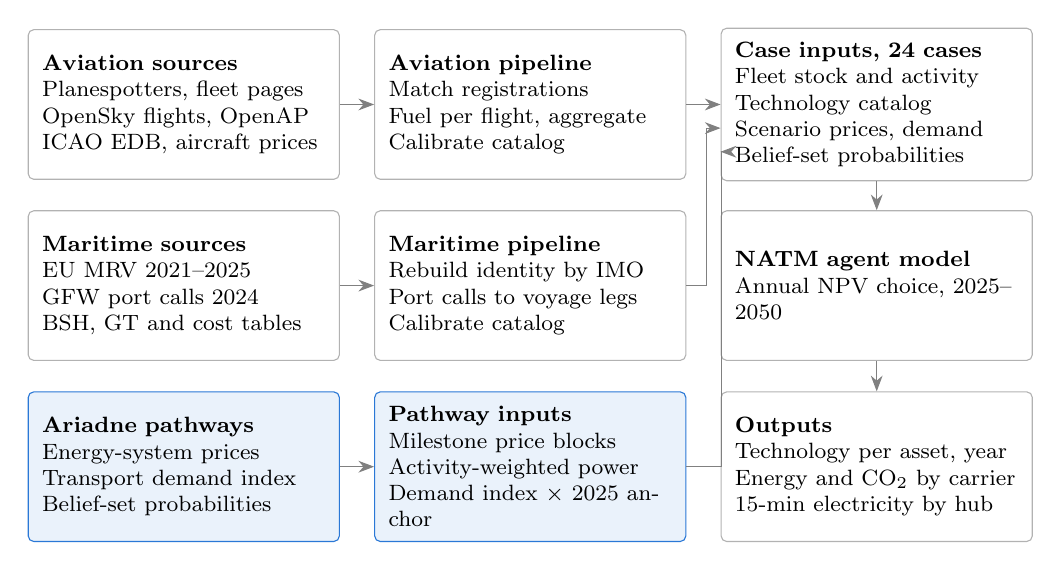
\begin{tikzpicture}[font=\footnotesize, box/.style={draw=gray!60, rounded corners=2pt, align=left, text width=3.6cm, inner sep=5pt, minimum height=1.9cm},
  path/.style={box, fill=c1!10, draw=c1}, arr/.style={-{Stealth[length=2mm]}, gray}]
\node[box] (as) at (0,0) {\textbf{Aviation sources}\\Planespotters, fleet pages\\OpenSky flights, OpenAP\\ICAO EDB, aircraft prices};
\node[box] (ms) at (0,-2.3) {\textbf{Maritime sources}\\EU MRV 2021--2025\\GFW port calls 2024\\BSH, GT and cost tables};
\node[path] (ar) at (0,-4.6) {\textbf{Ariadne pathways}\\Energy-system prices\\Transport demand index\\Belief-set probabilities};
\node[box] (ap) at (4.4,0) {\textbf{Aviation pipeline}\\Match registrations\\Fuel per flight, aggregate\\Calibrate catalog};
\node[box] (mp) at (4.4,-2.3) {\textbf{Maritime pipeline}\\Rebuild identity by IMO\\Port calls to voyage legs\\Calibrate catalog};
\node[path] (pi) at (4.4,-4.6) {\textbf{Pathway inputs}\\Milestone price blocks\\Activity-weighted power\\Demand index $\times$ 2025 anchor};
\node[box] (ci) at (8.8,0) {\textbf{Case inputs, 24 cases}\\Fleet stock and activity\\Technology catalog\\Scenario prices, demand\\Belief-set probabilities};
\node[box] (nm) at (8.8,-2.3) {\textbf{NATM agent model}\\Annual NPV choice, 2025--2050};
\node[box] (ou) at (8.8,-4.6) {\textbf{Outputs}\\Technology per asset, year\\Energy and CO$_2$ by carrier\\15-min electricity by hub};
\draw[arr] (as) -- (ap); \draw[arr] (ms) -- (mp); \draw[arr] (ar) -- (pi);
\draw[arr] (ap) -- (ci); \draw[arr] (mp.east) -- ++(0.25,0) |- ([yshift=-3mm]ci.west); \draw[arr] (pi.east) -- ++(0.45,0) |- ([yshift=-6mm]ci.west);
\draw[arr] (ci) -- (nm); \draw[arr] (nm) -- (ou);
\end{tikzpicture}
\caption{Dataset construction flow. Observed data fix the 2025 state through two sector pipelines; the Ariadne pathways (shaded) reach the model only through prices, demand indices and belief probabilities in each case's inputs.}
\label{fig:flow}
\end{figure}

Observed fleet, activity and fuel data fix the 2025 state through two sector pipelines; the Ariadne pathways reach the model only through prices, demand indices and belief probabilities in each case's inputs.

\subsection*{5.1 Aviation pipeline}
\addcontentsline{toc}{subsection}{5.1 Aviation pipeline}

\begin{enumerate}
\item{} \textbf{Filter fleet attributes.} Planespotters export (A1) → \texttt{planespotters\_\allowbreak{}germany\_\allowbreak{}commercial\_\allowbreak{}filtered.\allowbreak{}csv}, 787 rows: operator country Germany, commercial passenger or cargo operators.
\item{} \textbf{Match registrations} (\texttt{registration\_\allowbreak{}matching/\allowbreak{}build\_\allowbreak{}matches.\allowbreak{}py}). Each pasted registration is matched on operator + type family + delivery year and month, falling back to year only where a lease or transfer changed the delivery date. Results are bucketed as matched, ambiguous, zero candidates or too new for the 2023 snapshot (\texttt{matched.\allowbreak{}csv}, \texttt{ambiguous.\allowbreak{}csv}, \texttt{flagged\_\allowbreak{}*.\allowbreak{}csv}). Reason: the export carries attributes but no registration.
\item{} \textbf{Resolve ICAO24.} OpenSky database first (484/600), SkyLink second (+85) → \texttt{fleet\_\allowbreak{}stock\_\allowbreak{}with\_\allowbreak{}registrations\_\allowbreak{}and\_\allowbreak{}icao24.\allowbreak{}csv}.
\item{} \textbf{Pull flights} (\texttt{pull\_\allowbreak{}opensky\_\allowbreak{}flights.\allowbreak{}py}, \texttt{pull\_\allowbreak{}opensky\_\allowbreak{}flights\_\allowbreak{}delta.\allowbreak{}py}). Global \texttt{/\allowbreak{}flights/\allowbreak{}all} queries in 2-day windows (30 API credits per call) filtered to the ICAO24 set, resumable across three accounts → \texttt{opensky\_\allowbreak{}real\_\allowbreak{}flights\_\allowbreak{}matched.\allowbreak{}csv} (496,778) and \texttt{\_\allowbreak{}delta.\allowbreak{}csv} (628). Timestamps converted from Unix seconds to UTC.
\item{} \textbf{Model fuel and emissions} (\texttt{navaero\_\allowbreak{}transition\_\allowbreak{}model/\allowbreak{}aviation\_\allowbreak{}preprocessing/\allowbreak{}flight\_\allowbreak{}activity\_\allowbreak{}fuel.\allowbreak{}py}, OpenAP). Unsupported types mapped through a fallback table (\texttt{openap\_\allowbreak{}aircraft\_\allowbreak{}type\_\allowbreak{}mapping\_\allowbreak{}log.\allowbreak{}csv}); model objects cached and runs parallelised over 28 processes → \texttt{data/\allowbreak{}processed/\allowbreak{}aviation/\allowbreak{}openap\_\allowbreak{}flight\_\allowbreak{}fuel\_\allowbreak{}emissions.\allowbreak{}csv} (450,129 flights; kg fuel, MWh, kg pollutants). This 165 MB file is excluded from git.
\item{} \textbf{Aggregate per aircraft} → \texttt{aviation\_\allowbreak{}activity\_\allowbreak{}profiles.\allowbreak{}csv}; per-route and per-airport fuel demand files; fleet tables via \texttt{build\_\allowbreak{}real\_\allowbreak{}fleet\_\allowbreak{}stock.\allowbreak{}py}. Null operators on 259 flights re-mapped from the corrected fleet.
\item{} \textbf{Domestic share per registration} (\texttt{fix\_\allowbreak{}domestic\_\allowbreak{}international\_\allowbreak{}split.\allowbreak{}py}): distance-weighted share of flights with both endpoints in Germany, replacing a type-level average that had been applied to all 474 aircraft.
\item{} \textbf{Technology catalog}, in order: \texttt{fix\_\allowbreak{}aviation\_\allowbreak{}technology\_\allowbreak{}catalog.\allowbreak{}py} (rows and specifications), \texttt{fix\_\allowbreak{}aviation\_\allowbreak{}capex\_\allowbreak{}real\_\allowbreak{}prices.\allowbreak{}py} (CAPEX), \texttt{fix\_\allowbreak{}aviation\_\allowbreak{}emission\_\allowbreak{}factors.\allowbreak{}py} (EDB non-CO2 values, with the threshold change in \texttt{legacy\_\allowbreak{}weighted\_\allowbreak{}utility.\allowbreak{}py}), CO2 factor correction (0.89 → 0.2636 kg/kWh), \texttt{fix\_\allowbreak{}aviation\_\allowbreak{}kilometer\_\allowbreak{}per\_\allowbreak{}kwh.\allowbreak{}py} (efficiency), lifetimes.
\item{} \textbf{Install} into \texttt{data/\allowbreak{}input/\allowbreak{}baseline-passenger-transition/\allowbreak{}} and \texttt{baseline-cargo-transition/\allowbreak{}}, merge ultra-long into long-haul, then copy to the eight risk cases per sector.
\end{enumerate}

\subsection*{5.2 Maritime pipeline}
\addcontentsline{toc}{subsection}{5.2 Maritime pipeline}

\begin{enumerate}
\item{} \textbf{Verify identity} (\texttt{maritime/\allowbreak{}build/\allowbreak{}verify\_\allowbreak{}real\_\allowbreak{}identity.\allowbreak{}py}) → \texttt{real\_\allowbreak{}identity\_\allowbreak{}verified*.\allowbreak{}csv}: IMO-keyed join of M1 to MRV \texttt{Name}/\texttt{Company}, GFW name and flag, manual lookups.
\item{} \textbf{Merge MRV} (\texttt{merge\_\allowbreak{}real\_\allowbreak{}maritime\_\allowbreak{}fleet.\allowbreak{}py}): string errors coerced to null; per vessel, intensity from the latest reporting year with a value.
\item{} \textbf{Build fleet} (\texttt{build\_\allowbreak{}real\_\allowbreak{}maritime\_\allowbreak{}cargo\_\allowbreak{}fleet.\allowbreak{}py}): German-entity filter, GT segment rule (40,000), current technology (biofuel for the seven low-ratio newbuilds) → \texttt{real\_\allowbreak{}maritime\_\allowbreak{}cargo\_\allowbreak{}fleet\_\allowbreak{}stock.\allowbreak{}csv}, validated against BSH.
\item{} \textbf{Port calls and legs} (\texttt{maritime/\allowbreak{}AIS/\allowbreak{}fetch\_\allowbreak{}maritime.\allowbreak{}py}, \texttt{estimate\_\allowbreak{}route\_\allowbreak{}distances.\allowbreak{}ipynb}, \texttt{repair\_\allowbreak{}routes.\allowbreak{}py}): GFW 2024 port visits → consecutive-visit legs → \texttt{searoute} distances with great-circle check → \texttt{gfw\_\allowbreak{}route\_\allowbreak{}pairs\_\allowbreak{}2024\_\allowbreak{}with\_\allowbreak{}distances.\allowbreak{}csv}; leg fuel = MRV kg/n mile × distance → \texttt{maritime\_\allowbreak{}cargo\_\allowbreak{}route\_\allowbreak{}fuel\_\allowbreak{}demand.\allowbreak{}csv} (6,213 legs).
\item{} \textbf{Activity profile and merge} (\texttt{build\_\allowbreak{}maritime\_\allowbreak{}activity\_\allowbreak{}profiles.\allowbreak{}py}, \texttt{merge\_\allowbreak{}activity\_\allowbreak{}into\_\allowbreak{}fleet\_\allowbreak{}stock.\allowbreak{}py}): nm → km (× 1.852), MWh/n mile → kWh, main hub from AIS port time where available.
\item{} \textbf{Technology catalog}, in order: \texttt{expand\_\allowbreak{}technology\_\allowbreak{}catalog.\allowbreak{}py} (6 → 20 rows from the P01–P30 and R01–R07 taxonomy), \texttt{fix\_\allowbreak{}maritime\_\allowbreak{}technology\_\allowbreak{}costs.\allowbreak{}py} (ID-joined CAPEX, premia, bottom-up rows), \texttt{fix\_\allowbreak{}maritime\_\allowbreak{}kilometer\_\allowbreak{}per\_\allowbreak{}kwh\_\allowbreak{}and\_\allowbreak{}co2\_\allowbreak{}factor.\allowbreak{}py} (MRV-calibrated efficiency and CO2, IMO factors), lifetimes.
\item{} \textbf{Demand} (\texttt{fix\_\allowbreak{}maritime\_\allowbreak{}cargo\_\allowbreak{}demand\_\allowbreak{}scale.\allowbreak{}py}): 2025 capacity anchor × Ariadne shipping index (Section 7).
\end{enumerate}

\subsection*{5.3 Pathway price integration}
\addcontentsline{toc}{subsection}{5.3 Pathway price integration}

Prices enter as one value per pathway and milestone year (2030, 2035, 2040, 2045). The live inputs were traced column by column back to \texttt{forecasts\_\allowbreak{}df.\allowbreak{}csv}; the table gives the mapping as it stands now, including columns (tax-inclusive and blend prices) that were added to the forecast files after the first extraction.

{\footnotesize\setlength{\tabcolsep}{3pt}
\begin{longtable}{>{\raggedright\arraybackslash}p{0.151\linewidth}>{\raggedright\arraybackslash}p{0.151\linewidth}>{\raggedright\arraybackslash}p{0.151\linewidth}>{\raggedright\arraybackslash}p{0.151\linewidth}>{\raggedright\arraybackslash}p{0.151\linewidth}>{\raggedright\arraybackslash}p{0.151\linewidth}}
\toprule
\textbf{Model price variable (carrier)} & \textbf{Sector} & \textbf{Source column in P1/P2} & \textbf{Aggregation over the year} & \textbf{Example, AktuellePolitiken 2030, EUR/MWh} & \textbf{Status} \tabularnewline
\midrule
\endhead
primary, \texttt{kerosene} & Aviation & \texttt{kerosene\_\allowbreak{}mix\_\allowbreak{}DE} & Single value (flat) & 42.17 & [V] \tabularnewline
primary, \texttt{kerosene}, scoped to drop-in and e-kerosene technologies & Aviation & \texttt{fossil\_\allowbreak{}kerosene\_\allowbreak{}price\_\allowbreak{}EUR\_\allowbreak{}MWh} & Single value & 42.16 & [V] value; rationale [N] \tabularnewline
secondary, \texttt{saf} (HEFA) & Aviation & \texttt{SAF\_\allowbreak{}blended\_\allowbreak{}price\_\allowbreak{}EUR\_\allowbreak{}MWh} & Annual mean & 90.56 & [V] value; rationale [N] \tabularnewline
secondary, \texttt{e\_\allowbreak{}kerosene} (PtL) & Aviation & \texttt{ekerosene\_\allowbreak{}FT\_\allowbreak{}EU} & Single value & 42.15 & [V] \tabularnewline
primary, \texttt{hydrogen} & Both & \texttt{hydrogen\_\allowbreak{}with\_\allowbreak{}taxes} & Annual mean & 59.48 & [V] value; rationale [N] \tabularnewline
primary, \texttt{electricity} (hybrid-electric aircraft) & Aviation & \texttt{DA\_\allowbreak{}price\_\allowbreak{}EUR\_\allowbreak{}per\_\allowbreak{}MWh} (P2) & Weighted by observed quarter-hour activity & 10.73 & [V] \tabularnewline
primary, \texttt{marine\_\allowbreak{}diesel} & Maritime & \texttt{marinediesel\_\allowbreak{}mix\_\allowbreak{}DE} & Single value & 65.66 & [V] \tabularnewline
primary, \texttt{marine\_\allowbreak{}diesel}, scoped to biofuel technologies & Maritime & \texttt{fossil\_\allowbreak{}marinediesel\_\allowbreak{}price\_\allowbreak{}EUR\_\allowbreak{}MWh} & Single value & 42.16 & [V] value; rationale [N] \tabularnewline
secondary, \texttt{biofuel} (FAME) & Maritime & \texttt{marine\_\allowbreak{}blend\_\allowbreak{}price\_\allowbreak{}EUR\_\allowbreak{}MWh} & Annual mean & 90.56 & [V] value; rationale [N] \tabularnewline
tertiary, \texttt{biofuel} & Maritime & \texttt{biofuel\_\allowbreak{}BtL\_\allowbreak{}EU} & Single value & 42.15 & [V] \tabularnewline
primary, \texttt{lng} / \texttt{methanol} & Maritime & \texttt{lng\_\allowbreak{}mix\_\allowbreak{}DE} / \texttt{methanol\_\allowbreak{}synth\_\allowbreak{}DE} & Single value / annual mean & 24.01 / 89.46 & [V] \tabularnewline
primary, \texttt{electricity} (battery ship) & Maritime & \texttt{DE\_\allowbreak{}DA\_\allowbreak{}price\_\allowbreak{}with\_\allowbreak{}taxes} & Annual mean & 24.20 & [V] value; rationale [N] \tabularnewline
secondary, \texttt{electricity} (hybrid assist) & Maritime & \texttt{DA\_\allowbreak{}price\_\allowbreak{}EUR\_\allowbreak{}per\_\allowbreak{}MWh} (P2) & Weighted by observed AIS port-time activity & 10.32 & [V] \tabularnewline
primary, \texttt{ammonia} & Maritime & P4 midpoint, not P1 & Fixed series, all pathways & 151.4 (2030) & [V] \tabularnewline
\bottomrule
\end{longtable}}

For the activity-weighted electricity prices (\texttt{price\_\allowbreak{}signal/\allowbreak{}apply\_\allowbreak{}consumption\_\allowbreak{}weighted\_\allowbreak{}price.\allowbreak{}py}):

\[
\bar{p}_{c,p,y} = \frac{\sum_k w_k \, p_{c,p,y}(\tau_k)}{\sum_k w_k}
\]

where \emph{k} indexes the 672 quarter-hours of a week, \emph{p}(τₖ) is the day-ahead price in that slot and \emph{w}ₖ the observed share of activity in it (OpenSky departure times for aviation, GFW port-visit times for maritime). All values are divided by 1,000 to give EUR/kWh. Ammonia: midpoint USD/GJ ÷ 277.78 kWh/GJ ÷ 1.1652 USD/EUR.

An earlier extraction weighted hydrogen and methanol by individual refuelling events (flight departures and voyage arrivals). Those values were later superseded by the annual means in the table; the event-weighted variant is documented in the session record but is not what the current inputs contain [V].

\subsection*{5.4 Unit conversions used}
\addcontentsline{toc}{subsection}{5.4 Unit conversions used}

{\small\setlength{\tabcolsep}{3pt}
\begin{longtable}{>{\raggedright\arraybackslash}p{0.478\linewidth}>{\raggedright\arraybackslash}p{0.478\linewidth}}
\toprule
\textbf{Conversion} & \textbf{Factor} \tabularnewline
\midrule
\endhead
Nautical mile → km & 1.852 \tabularnewline
Jet A-1 kg → kWh & 11.986 (43.15 MJ/kg) for CO2 factor; OpenAP implied \textasciitilde{}11.94 for energy \tabularnewline
LNG, methanol kg → kWh & 13.33 (48,000 kJ/kg), 5.53 (19,900 kJ/kg) \tabularnewline
GJ → kWh & 277.78 \tabularnewline
USD → EUR & Annual average of quote year: 2001 1.117, 2004 0.804, 2007 0.729, 2011 0.718, 2012 0.778, 2021 0.846, 2022 0.951; 2026 spot 0.858 \tabularnewline
EUR/MWh → EUR/kWh & ÷ 1,000 \tabularnewline
\bottomrule
\end{longtable}}

\section*{6. Relationship with technology adoption and investment modelling}
\addcontentsline{toc}{section}{6. Relationship with technology adoption and investment modelling}

The baseline datasets are the initial state of NATM, an agent-based model in which each operator (11 passenger airlines, 3 cargo airlines, 77 shipping companies) decides each year, asset by asset, which technology to invest in when an asset is due for replacement or when demand exceeds fleet capacity. Everything downstream of the inputs below is computed by the model.

\subsection*{6.1 Inputs, assumptions and endogenous outputs}
\addcontentsline{toc}{subsection}{6.1 Inputs, assumptions and endogenous outputs}

{\small\setlength{\tabcolsep}{3pt}
\begin{longtable}{>{\raggedright\arraybackslash}p{0.315\linewidth}>{\raggedright\arraybackslash}p{0.315\linewidth}>{\raggedright\arraybackslash}p{0.315\linewidth}}
\toprule
\textbf{Category} & \textbf{Item} & \textbf{Where it lives} \tabularnewline
\midrule
\endhead
\textbf{Input data} & Asset list with type, operator, segment, age, seats or payload, observed activity and energy & \texttt{*\_\allowbreak{}fleet\_\allowbreak{}stock.\allowbreak{}csv}, \texttt{aviation\_\allowbreak{}activity\_\allowbreak{}profiles.\allowbreak{}csv} \tabularnewline
Input data & Technology rows: CAPEX, lifetime, efficiency, emission factors, energy carriers, blend limits, entry year, range, seats/payload & \texttt{*\_\allowbreak{}technology\_\allowbreak{}catalog.\allowbreak{}csv} \tabularnewline
Input data & Pathway prices, demand, SAF/PtL shares; shared carbon price, subsidies, mandates, availability, market shares, load factors, fares and freight rates & \texttt{*\_\allowbreak{}scenario.\allowbreak{}csv} \tabularnewline
Input data & Belief-set probabilities over the six pathways & \texttt{ambiguity\_\allowbreak{}probabilities.\allowbreak{}csv} \tabularnewline
\textbf{Model assumptions} & Replacement at end of technical life; early replacement only for conventional assets within a policy-driven window and after a minimum holding period & \texttt{fleet.\allowbreak{}py}, \texttt{scorer.\allowbreak{}py} \tabularnewline
Model assumptions & Existing assets fly at most their observed distance (utilisation ≤ 1); new assets added only to close a capacity gap & agent classes, \texttt{scorer.\allowbreak{}py::\_\allowbreak{}add\_\allowbreak{}growth\_\allowbreak{}assets} \tabularnewline
Model assumptions & Decision criterion = NPV under the pathway probabilities and the case's risk attitude & \texttt{ambiguity\_\allowbreak{}aware\_\allowbreak{}utility.\allowbreak{}py} \tabularnewline
Model assumptions & New assets copy their segment's template route profile; renewal never changes route or hub & \texttt{fleet.\allowbreak{}py::apply\_\allowbreak{}technology} \tabularnewline
Model assumptions & Unlisted availability flags default to available & \texttt{legacy\_\allowbreak{}weighted\_\allowbreak{}utility.\allowbreak{}py::is\_\allowbreak{}candidate\_\allowbreak{}available} \tabularnewline
\textbf{Endogenous outputs} & Technology chosen per asset and year; timing of replacements; number and technology of growth assets & \texttt{aircraft.\allowbreak{}csv} / vessel outputs per case \tabularnewline
Endogenous outputs & Energy by carrier, CO2, ETS cost, NPV and costs per asset and year & \texttt{*\_\allowbreak{}energy\_\allowbreak{}emissions.\allowbreak{}csv} \tabularnewline
Endogenous outputs & Electricity, hydrogen and PtL demand by airport or port, 15-minute profiles & \texttt{data/\allowbreak{}processed/\allowbreak{}electricity\_\allowbreak{}15min/\allowbreak{}} \tabularnewline
\bottomrule
\end{longtable}}

\subsection*{6.2 How the baseline enters the decision}
\addcontentsline{toc}{subsection}{6.2 How the baseline enters the decision}

\textbf{Replacement opportunities.} For asset \emph{i} with age \emph{a}ᵢ and technology lifetime \emph{L}: first replacement year = 2025 + (\emph{L} − \emph{a}ᵢ); after a switch, year + \emph{L}. Lifetimes are 25 years (passenger aircraft, all vessels) and 33 years (freighters). Because of observed ages, 52 passenger aircraft, 4 freighters and 50 vessels are due at or near the start.

\textbf{Candidate set.} A technology is eligible if it serves the asset's segment and stage length, has reached its service-entry year, and is not switched off by a pathway availability flag (Section 3.4 and 4.6 list entry years).

\textbf{Net present value} per candidate and pathway \emph{p} (\texttt{scorer.\allowbreak{}py::calc\_\allowbreak{}payback\_\allowbreak{}year}):

\[
\mathrm{NPV}_{j,p} = -C_j + \sum_{t=1}^{L_j} \frac{R_{t} - \big(c^{E}_{p,t} E_{j,t} + \pi_{t} \max(0, Q^{CO_2}_{j,t} - A_{t})\big) - M_{j,t} - \delta_j C_j}{(1+r_j)^t} + \frac{V_j}{(1+r_j)^{L_j}}
\]

\emph{C} = CAPEX; \emph{R} = revenue (seats or payload × load factor × distance × fare or freight rate); \emph{c}ᴱ\emph{E} = energy cost from pathway prices and the mandated primary/secondary split; π = carbon price; \emph{A} = free ETS allocation; \emph{M} = maintenance and fixed operating shares; δ = depreciation share; \emph{V} = residual value; \emph{r} = technology discount rate (0.07–0.09 in the aviation catalog).

\textbf{Risk and ambiguity.} Each candidate is scored under all six pathways, with outcome probabilities \emph{q} from the belief-set matrix. Risk-neutral cases use the expected NPV under one pinned belief set; the two risk-averse cases use the worst case over probability bounds spanned by all six belief sets, either the worst-case expected NPV (\texttt{worst\_\allowbreak{}case\_\allowbreak{}expected\_\allowbreak{}utility}) or the worst-case expected shortfall (\texttt{worst\_\allowbreak{}case\_\allowbreak{}expected\_\allowbreak{}shortfall}). Each case then realises one pathway (\texttt{realized\_\allowbreak{}scenario\_\allowbreak{}id}) for prices and demand.

\textbf{Energy carriers.} Each technology row names a primary and, where relevant, secondary carrier (e.g. kerosene + HEFA-SAF, kerosene + PtL, marine diesel + FAME, LNG + diesel pilot, hydrogen, electricity); energy use per asset is the observed distance × utilisation ÷ the row's efficiency, split by the mandated blend share.

\subsection*{6.3 Relationship with the earlier published work}
\addcontentsline{toc}{subsection}{6.3 Relationship with the earlier published work}

NATM is the model behind Khanra, Prabhu and Wietschel (2025), the repository's preferred citation. Before this dataset work, the case folders held illustrative inputs: for example a 4-vessel maritime fleet, an 8-row passenger and a 6-row cargo technology catalog with round-number parameters, and placeholder demand and prices for Germany, France and Ireland. Whether those placeholders were the published paper's inputs could not be established from the files [N].

{\small\setlength{\tabcolsep}{3pt}
\begin{longtable}{>{\raggedright\arraybackslash}p{0.315\linewidth}>{\raggedright\arraybackslash}p{0.315\linewidth}>{\raggedright\arraybackslash}p{0.315\linewidth}}
\toprule
\textbf{Element} & \textbf{Reused} & \textbf{Updated for this paper} \tabularnewline
\midrule
\endhead
Agent-based structure, technology-row schema, NPV and replacement logic & Yes & Ambiguity-aware decision under six pathways; utilisation cap on existing assets \tabularnewline
Maritime vessel list and cost table from earlier research (M1, M10) & Partly: IMO list as a starting point; cost table used for CAPEX & Identity rebuilt from IMO; fleet expanded to 131 and validated against BSH \tabularnewline
Aviation fleet, activity and fuel & No surviving earlier dataset & Built new from Planespotters, operator pages, OpenSky and OpenAP \tabularnewline
Technology catalogs & Original rows used as the starting template & CAPEX, efficiency, emission factors, lifetimes and new technologies replaced with sourced values \tabularnewline
Environmental-utility thresholds & Original scheme & Recalibrated to EDB-based values (diagnostic only) \tabularnewline
Countries and corridors & Original Germany/France/Ireland setup & France and Ireland removed; corridor table now empty \tabularnewline
\bottomrule
\end{longtable}}

\section*{7. Integration with the six Ariadne transition pathways}
\addcontentsline{toc}{section}{7. Integration with the six Ariadne transition pathways}

All six pathways start from the identical 2025 fleet, activity, technology catalog and demand anchor; they diverge only through energy-carrier prices, passenger-aviation and shipping demand, and aviation SAF/PtL blend shares [V]. Carbon prices, subsidies, mandates for shipping, availability flags, market shares, fares and cargo-aviation demand are shared across pathways.

\subsection*{7.1 Naming and case structure}
\addcontentsline{toc}{subsection}{7.1 Naming and case structure}

{\footnotesize\setlength{\tabcolsep}{3pt}
\begin{longtable}{>{\raggedright\arraybackslash}p{0.184\linewidth}>{\raggedright\arraybackslash}p{0.184\linewidth}>{\raggedright\arraybackslash}p{0.184\linewidth}>{\raggedright\arraybackslash}p{0.184\linewidth}>{\raggedright\arraybackslash}p{0.184\linewidth}}
\toprule
\textbf{Pathway} & \textbf{Model scenario id} & \textbf{Code in demand table (P3)} & \textbf{Belief set} & \textbf{Risk-neutral case pinned to it} \tabularnewline
\midrule
\endhead
AktuellePolitiken & \texttt{aktuellepolitiken} & ExPol & B\_AktuellePolitiken & yes \tabularnewline
FokusStrom & \texttt{fokusstrom} & Elek & B\_FokusStrom & yes \tabularnewline
FokusH2 & \texttt{fokusH2} & H2 & B\_FokusH2 & yes \tabularnewline
Technologiemix & \texttt{technologiemix} & Mix & B\_Technologiemix & yes \tabularnewline
HoheNachfrage & \texttt{hohenachfrage} & NFhoch & B\_HoheNachfrage & yes \tabularnewline
NiedrigeNachfrage & \texttt{niedrigenachfrage} & NFniedrig & B\_NachfrageNiedrig & yes \tabularnewline
\bottomrule
\end{longtable}}

Each belief set gives its focal pathway probability 0.5625 or 0.625 and spreads the rest (0.0625 or 0.125 each) over the others (P5). Per sector there are eight cases: six risk-neutral cases, each pinned to one belief set and realising that pathway, and two ambiguity-averse cases (worst-case mean and worst-case expected shortfall) that use bounds over all six belief sets [V].

The six pathways are the scenarios of the Ariadne scenario report \citep{luderer2025}: a reference with existing policies only (code ExPol; AktuellePolitiken here), three technology-focus scenarios that reach climate neutrality in 2045 (Fokus Strom, Fokus Wasserstoff and Technologiemix; codes Elek, H2 and Mix), and two demand variants (Hohe Nachfrage and Niedrige Nachfrage; codes NFhoch and NFniedrig). The match between the codes in P3 and the report's scenario names is inferred from the names; it is not documented in the project files [A].

\subsection*{7.2 What varies by pathway}
\addcontentsline{toc}{subsection}{7.2 What varies by pathway}

{\footnotesize\setlength{\tabcolsep}{3pt}
\begin{longtable}{>{\raggedright\arraybackslash}p{0.184\linewidth}>{\raggedright\arraybackslash}p{0.184\linewidth}>{\raggedright\arraybackslash}p{0.184\linewidth}>{\raggedright\arraybackslash}p{0.184\linewidth}>{\raggedright\arraybackslash}p{0.184\linewidth}}
\toprule
\textbf{Input} & \textbf{Aviation passenger} & \textbf{Aviation cargo} & \textbf{Maritime cargo} & \textbf{Derivation} \tabularnewline
\midrule
\endhead
Fuel and electricity prices & Varies & Varies & Varies & P1/P2 per pathway and milestone (Section 5.3) [V] \tabularnewline
Transport demand & Varies & Shared & Varies & P3 index on the 2025 anchor (7.3) [V]; cargo aviation [N] \tabularnewline
SAF and PtL blend shares (\texttt{saf\_\allowbreak{}mandate}) & Varies & Varies & — & Present per pathway; derivation not recorded [N] \tabularnewline
Carbon price, EUR/t CO2 & 35 (2025), 105 (2030), 180 (2035–2050) & same & 28, 78, 152 (\texttt{carbon\_\allowbreak{}tax}) & Shared [A; origin N] \tabularnewline
Clean-fuel subsidy, adoption mandate & 8\% → 22\%; 3\% → 28\% & shared & biofuel mandate 2\% → 23\% & Shared [A; origin N] \tabularnewline
Ammonia price & — & — & 176.4 (2025), 151.4 (2030), 144.6 (2035–2050) EUR/MWh & Shared, P4 [V] \tabularnewline
Market shares, load factors, fares, freight rates, availability & Shared & Shared & Shared & Market shares = operator share of 2025 segment seat-km (passenger, verified) or vessel count (maritime, verified); cargo [N] \tabularnewline
\bottomrule
\end{longtable}}

\subsection*{7.3 Demand by pathway}
\addcontentsline{toc}{subsection}{7.3 Demand by pathway}

Passenger aviation combines the domestic and international P3 trajectories with each segment's observed domestic share δₛ (short 0.11303, medium 0.011604, long 0.001344):

\[
P_{s,p,t} = P_{s,2025} \left[ \delta_s \frac{\mathrm{Dom}_{p,t}}{\mathrm{Dom}_{p,2025}} + (1-\delta_s) \frac{\mathrm{Int}_{p,t}}{\mathrm{Int}_{p,2025}} \right]
\]

Example, FokusH2, short segment, 2035: 29.77 × [0.113 × (4.163/7.395) + 0.887 × (169.51/201.85)] = 24.07 billion seat-km (−19.2\%).

Maritime scales the 2025 capacity anchor by the international-shipping index, with the regional/deepsea split fixed at 16.21/83.79\%:

\[
Q_{g,p,t} = Q_{g,2025} \, \frac{S_{p,t}}{S_{p,2025}}
\]

Example, FokusH2, regional, 2050: 64.32 × (772.85/1147.75) = 43.31 billion tkm (−32.7\%).

The two sectors fill years between milestones differently [V]. Maritime interpolates linearly between all six milestones to 2050. Passenger aviation holds 2025 for 2026–2029, 2030 for 2031–2034, and the 2035 value for all of 2035–2050, so the 2040–2050 P3 values (e.g. FokusH2 international 149.2 → 145.1 bn pkm) are not used. Cargo-aviation demand is identical in all pathways and grows +14\% to 2030 and +30\% to 2035, then stays flat [N]. The Ariadne demand data \citep{luderer2025} does provide per-pathway values for every milestone year for both passenger and cargo aviation, so both gaps come from how the inputs were built, not from missing data (Section 8, item 2).

\begin{figure}[htbp]
\centering
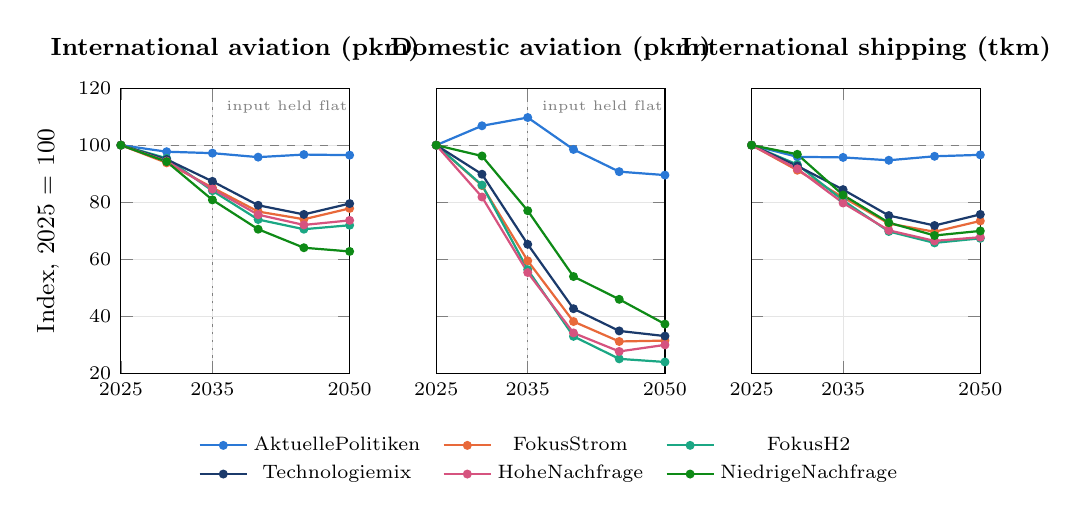
\begin{tikzpicture}
\begin{groupplot}[group style={group size=3 by 1, horizontal sep=1.1cm, y descriptions at=edge left},
  width=0.37\linewidth, height=5.2cm, ymin=20, ymax=120, xmin=2025, xmax=2050,
  xtick={2025,2035,2050}, ytick={20,40,60,80,100,120}, grid=major, grid style={gray!20},
  tick label style={font=\scriptsize, /pgf/number format/1000 sep={}}, title style={font=\small\bfseries},
  every axis plot/.append style={thick, mark=*, mark size=1.2pt}, ylabel={Index, 2025 = 100}, ylabel style={font=\small},
  legend style={font=\scriptsize, draw=none, legend columns=3, /tikz/every even column/.append style={column sep=6pt}}]
\nextgroupplot[title={International aviation (pkm)}]
\addplot[gray, dashed, thin, mark=none, forget plot] coordinates {(2025,100) (2050,100)};
\addplot[gray, dotted, thin, mark=none, forget plot] coordinates {(2035,20) (2035,120)};
\node[font=\tiny, anchor=north west, gray] at (axis cs:2035.5,119) {input held flat};
\addplot[c1] coordinates {(2025,100.0) (2030,97.7) (2035,97.2) (2040,95.8) (2045,96.7) (2050,96.5)};
\addplot[c2] coordinates {(2025,100.0) (2030,93.8) (2035,85.1) (2040,76.7) (2045,74.0) (2050,77.8)};
\addplot[c3] coordinates {(2025,100.0) (2030,95.4) (2035,84.0) (2040,73.9) (2045,70.5) (2050,71.9)};
\addplot[c4] coordinates {(2025,100.0) (2030,95.0) (2035,87.3) (2040,78.9) (2045,75.7) (2050,79.5)};
\addplot[c5] coordinates {(2025,100.0) (2030,94.4) (2035,84.6) (2040,75.6) (2045,72.0) (2050,73.6)};
\addplot[c6] coordinates {(2025,100.0) (2030,94.2) (2035,80.8) (2040,70.5) (2045,64.0) (2050,62.7)};
\nextgroupplot[title={Domestic aviation (pkm)}, legend to name=demleg]
\addplot[gray, dashed, thin, mark=none, forget plot] coordinates {(2025,100) (2050,100)};
\addplot[gray, dotted, thin, mark=none, forget plot] coordinates {(2035,20) (2035,120)};
\node[font=\tiny, anchor=north west, gray] at (axis cs:2035.5,119) {input held flat};
\addplot[c1] coordinates {(2025,100.0) (2030,106.8) (2035,109.7) (2040,98.5) (2045,90.7) (2050,89.5)};
\addlegendentry{AktuellePolitiken}
\addplot[c2] coordinates {(2025,100.0) (2030,85.8) (2035,59.4) (2040,38.1) (2045,31.1) (2050,31.4)};
\addlegendentry{FokusStrom}
\addplot[c3] coordinates {(2025,100.0) (2030,86.0) (2035,56.3) (2040,32.9) (2045,25.0) (2050,23.9)};
\addlegendentry{FokusH2}
\addplot[c4] coordinates {(2025,100.0) (2030,89.8) (2035,65.2) (2040,42.6) (2045,34.8) (2050,33.0)};
\addlegendentry{Technologiemix}
\addplot[c5] coordinates {(2025,100.0) (2030,81.8) (2035,55.3) (2040,34.1) (2045,27.6) (2050,29.9)};
\addlegendentry{HoheNachfrage}
\addplot[c6] coordinates {(2025,100.0) (2030,96.2) (2035,77.0) (2040,53.9) (2045,45.9) (2050,37.2)};
\addlegendentry{NiedrigeNachfrage}
\nextgroupplot[title={International shipping (tkm)}]
\addplot[gray, dashed, thin, mark=none, forget plot] coordinates {(2025,100) (2050,100)};
\addplot[c1] coordinates {(2025,100.0) (2030,95.9) (2035,95.7) (2040,94.7) (2045,96.1) (2050,96.6)};
\addplot[c2] coordinates {(2025,100.0) (2030,91.2) (2035,81.7) (2040,72.5) (2045,69.6) (2050,73.4)};
\addplot[c3] coordinates {(2025,100.0) (2030,93.2) (2035,80.6) (2040,69.7) (2045,65.7) (2050,67.3)};
\addplot[c4] coordinates {(2025,100.0) (2030,92.7) (2035,84.4) (2040,75.3) (2045,71.8) (2050,75.7)};
\addplot[c5] coordinates {(2025,100.0) (2030,91.7) (2035,79.7) (2040,70.1) (2045,66.4) (2050,67.7)};
\addplot[c6] coordinates {(2025,100.0) (2030,96.8) (2035,82.5) (2040,72.8) (2045,68.3) (2050,69.9)};
\end{groupplot}
\node at ($(group c2r1.south)+(0,-1.1cm)$) {\pgfplotslegendfromname{demleg}};
\end{tikzpicture}
\caption{Ariadne transport-service projections for Germany by pathway, 2025--2050, indexed to 2025 = 100 (P3; \citealp{luderer2025}). The dotted line at 2035 marks where the passenger-aviation model input stops following the projection and is held flat. By 2050 the international-aviation index ranges from 63 (NiedrigeNachfrage) to 97 (AktuellePolitiken), domestic aviation from 24 (FokusH2) to 89, and shipping from 67 (FokusH2) to 97.}
\label{fig:demand}
\end{figure}

The source projections diverge mainly after 2030. By 2050 the international-aviation index ranges from 63 (NiedrigeNachfrage) to 97 (AktuellePolitiken), domestic aviation from 24 (FokusH2) to 89, and shipping from 67 (FokusH2) to 97. The dotted line marks where the passenger model input stops following the projection.

\subsection*{7.4 Prices by pathway}
\addcontentsline{toc}{subsection}{7.4 Prices by pathway}

Price milestones are held in blocks: 2025–2034 take 2030, 2035–2039 take 2035, 2040–2044 take 2040, 2045–2050 take 2045 [V]. Kerosene, hydrogen and electricity by pathway are shown in Figure~\ref{fig:prices}.

\begin{figure}[htbp]
\centering
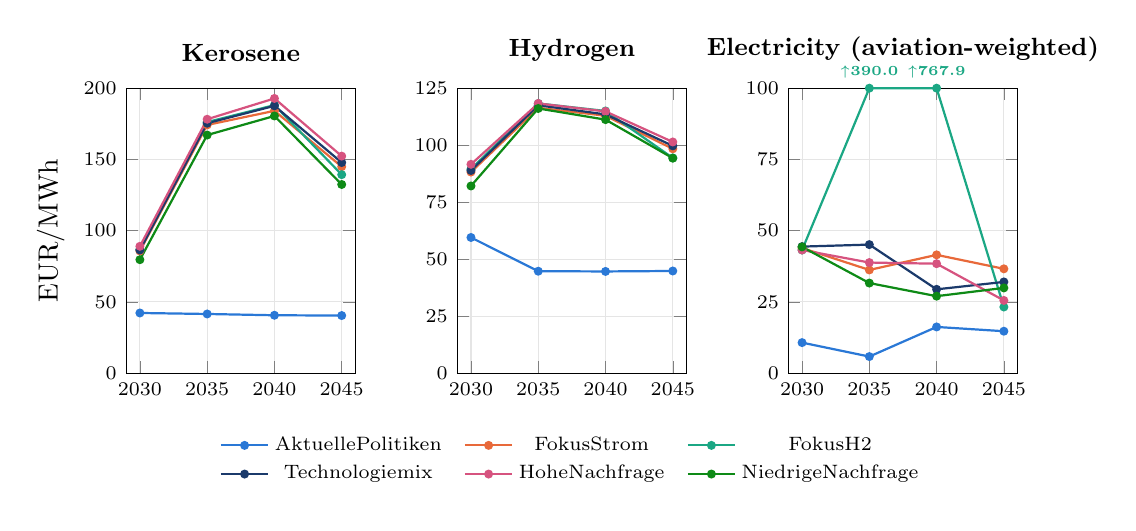
\begin{tikzpicture}
\begin{groupplot}[group style={group size=3 by 1, horizontal sep=1.3cm},
  width=0.37\linewidth, height=5.2cm, xmin=2029, xmax=2046, ymin=0,
  xtick={2030,2035,2040,2045}, grid=major, grid style={gray!20}, clip=false,
  tick label style={font=\scriptsize, /pgf/number format/1000 sep={}}, title style={font=\small\bfseries},
  every axis plot/.append style={thick, mark=*, mark size=1.2pt},
  legend style={font=\scriptsize, draw=none, legend columns=3, /tikz/every even column/.append style={column sep=6pt}}]
\nextgroupplot[title={Kerosene}, ymax=200, ytick={0,50,100,150,200}, ylabel={EUR/MWh}]
\addplot[c1] coordinates {(2030,42.2) (2035,41.5) (2040,40.6) (2045,40.4)};
\addplot[c2] coordinates {(2030,85.7) (2035,174.2) (2040,184.1) (2045,144.9)};
\addplot[c3] coordinates {(2030,86.9) (2035,176.2) (2040,188.1) (2045,139.3)};
\addplot[c4] coordinates {(2030,86.4) (2035,175.4) (2040,187.6) (2045,147.8)};
\addplot[c5] coordinates {(2030,89.0) (2035,178.2) (2040,192.8) (2045,152.3)};
\addplot[c6] coordinates {(2030,79.6) (2035,167.1) (2040,180.5) (2045,132.4)};
\nextgroupplot[title={Hydrogen}, ymax=125, ytick={0,25,50,75,100,125}, legend to name=prileg]
\addplot[c1] coordinates {(2030,59.5) (2035,44.7) (2040,44.6) (2045,44.8)};
\addlegendentry{AktuellePolitiken}
\addplot[c2] coordinates {(2030,88.2) (2035,116.4) (2040,112.9) (2045,98.4)};
\addlegendentry{FokusStrom}
\addplot[c3] coordinates {(2030,89.5) (2035,118.3) (2040,115.0) (2045,94.4)};
\addlegendentry{FokusH2}
\addplot[c4] coordinates {(2030,88.9) (2035,117.5) (2040,113.5) (2045,99.7)};
\addlegendentry{Technologiemix}
\addplot[c5] coordinates {(2030,91.6) (2035,118.3) (2040,114.8) (2045,101.4)};
\addlegendentry{HoheNachfrage}
\addplot[c6] coordinates {(2030,82.1) (2035,116.1) (2040,111.2) (2045,94.3)};
\addlegendentry{NiedrigeNachfrage}
\nextgroupplot[title={Electricity (aviation-weighted)}, ymax=100, ytick={0,25,50,75,100}]
\addplot[c1] coordinates {(2030,10.7) (2035,5.8) (2040,16.2) (2045,14.7)};
\addplot[c2] coordinates {(2030,43.9) (2035,36.2) (2040,41.5) (2045,36.6)};
\addplot[c3] coordinates {(2030,43.2) (2035,100.0) (2040,100.0) (2045,23.2)};
\node[c3, font=\tiny\bfseries, anchor=south] at (axis cs:2035,100) {$\uparrow$390.0};
\node[c3, font=\tiny\bfseries, anchor=south] at (axis cs:2040,100) {$\uparrow$767.9};
\addplot[c4] coordinates {(2030,44.4) (2035,45.1) (2040,29.4) (2045,32.0)};
\addplot[c5] coordinates {(2030,43.2) (2035,38.8) (2040,38.4) (2045,25.5)};
\addplot[c6] coordinates {(2030,44.3) (2035,31.6) (2040,27.0) (2045,29.9)};
\end{groupplot}
\node at ($(group c2r1.south)+(0,-1.1cm)$) {\pgfplotslegendfromname{prileg}};
\end{tikzpicture}
\caption{Energy-carrier prices in the live model inputs by pathway at the milestone years (EUR/MWh; source file \texttt{data/\allowbreak input/\allowbreak baseline-passenger-transition/\allowbreak aviation\_scenario.csv}). Each value holds for its five-year block. Electricity values above the axis are printed (FokusH2: 390.0 in 2035 and 767.9 in 2040). Kerosene costs about twice the AktuellePolitiken level in 2030 and about 4.6 times it in 2040.}
\label{fig:prices}
\end{figure}

AktuellePolitiken keeps fossil kerosene near 40–42 EUR/MWh throughout, while the five decarbonisation pathways roughly double it by 2030 and quadruple it by 2040, as scarcity and blending costs enter the oil-product price in the energy-system model.

\subsection*{7.5 Use for 2030–2050 assessments}
\addcontentsline{toc}{subsection}{7.5 Use for 2030–2050 assessments}

The simulation runs annually from 2025 to 2050. Milestone years 2030, 2035, 2040 and 2045 carry pathway-specific prices taken directly from the energy-system results; 2050 repeats 2045 prices. Results for any year are therefore traceable to one milestone block of prices, one demand trajectory and the fleet state the model has built up to that year. Pathway-specific electricity, hydrogen and PtL demand per airport and port is exported per case at 15-minute resolution (Section 3.7) for return to the energy-system or market assessment; which case's output is passed onward is decided outside NATM [N].

\section*{8. Limitations, open gaps and items that cannot be reconstructed}
\addcontentsline{toc}{section}{8. Limitations, open gaps and items that cannot be reconstructed}

Nineteen items need either a disclosure in the paper or a fix before submission. Items 1–7 can change results; items 8–13 are disclosure-level simplifications; items 14–19 are provenance gaps that need the original download or author record.

{\footnotesize\setlength{\tabcolsep}{3pt}
\begin{longtable}{>{\raggedright\arraybackslash}p{0.028\linewidth}>{\raggedright\arraybackslash}p{0.223\linewidth}>{\raggedright\arraybackslash}p{0.223\linewidth}>{\raggedright\arraybackslash}p{0.223\linewidth}>{\raggedright\arraybackslash}p{0.223\linewidth}}
\toprule
\textbf{\#} & \textbf{Item} & \textbf{Effect} & \textbf{Status} & \textbf{Suggested action} \tabularnewline
\midrule
\endhead
1 & 119 passenger aircraft have haul segment \emph{medium} but technology \texttt{kerosene\_\allowbreak{}short} & Demand and replacement candidates are drawn from a different segment than the aircraft's current technology & [V] & Re-assign \texttt{current\_\allowbreak{}technology} from the haul segment, or document the rule \tabularnewline
2 & Passenger demand holds the 2035 value for 2035–2050 and cargo demand is shared across pathways, although the Ariadne data has per-pathway, per-year values for both; maritime interpolates all milestones & Pathway differences in aviation demand are lost: passenger after 2035, cargo in every year & [V] & Build passenger and cargo aviation demand from the Ariadne pathway values for every milestone year, interpolated as for maritime \tabularnewline
3 & Passenger demand anchor is seat-km (no load factor) & Demand equals 2025 capacity, so growth assets appear only if demand rises above observed capacity & [A] & State explicitly; consider a load-factor adjustment \tabularnewline
4 & Electricity price spikes in FokusH2: 390 (2035) and 768 EUR/MWh (2040), aviation-weighted & Electric options look prohibitive in those blocks & [V] & Check the source series for scarcity hours \tabularnewline
5 & \texttt{efficient\_\allowbreak{}turbofan} gets 20\% lower CO2 and non-CO2 factors but the same efficiency as kerosene & Its fuel saving reduces carbon cost but not energy cost & [V] & Move the 20\% into \texttt{kilometer\_\allowbreak{}per\_\allowbreak{}kwh} and restore kerosene emission factors \tabularnewline
6 & SAF/PtL shares (\texttt{saf\_\allowbreak{}mandate}) fall to 0 from 2035 in AktuellePolitiken & Current-policy case loses blending after 2035 & [N] & Confirm against the pathway source \tabularnewline
7 & Ammonia price fixed after 2035 although the source table gives 2040–2050 midpoints (44.5, 42.3, 40.0 USD/GJ) & Ammonia slightly too expensive after 2035 & [V] & Extend the series \tabularnewline
8 & Methanol and ammonia are not converted into upstream electricity or hydrogen demand & Power-to-X demand for shipping is understated & [V] & Add conversion efficiencies \tabularnewline
9 & 91 of 131 vessels default to Hamburg as main hub & Spatial port attribution only; totals unaffected & [A] & Disclose \tabularnewline
10 & Observation windows (Aug 2025–Aug 2026 flights; 2024 voyages; MRV 2021–2025) assigned to 2025 without scaling & Baseline year is a composite & [A] & Disclose \tabularnewline
11 & 50 vessels, 52 passenger aircraft and 4 freighters are at or beyond lifetime in 2025 & Large immediate replacement wave & [V] & Disclose; test sensitivity to lifetime \tabularnewline
12 & Exclusions: DH8D and D328 types (incl. 9 Private Wings aircraft), \textasciitilde{}31 unresolved registrations; cargo fleet 74 vs Eurostat 119 & Fleet slightly below official counts & [V] & Disclose with the operator-level reconciliation \tabularnewline
13 & Cost proxies and estimates: Boeing types priced at Airbus equivalents; list and market values mixed; general cargo and heavy load ships on the tanker cost curve; hybrid-electric aircraft (EUR 38 M), efficient turbofan (+8\%), rotor-sail counts and PTI motor sizes are estimates & CAPEX uncertainty, largest for new technologies & [A] & Sensitivity analysis on CAPEX \tabularnewline
14 & Ariadne source of P1, P3 and the SAF shares: report, model and data version & Citability & [N] & Add citation and version \tabularnewline
15 & Eurostat dataset code, BSH edition, \emph{Verkehr in Zahlen} edition, OpenAP version, download dates & Reproducibility & [N] & Record from original downloads \tabularnewline
16 & Origin of the ammonia cost table (P4) and the belief-set probabilities (P5) & Citability & [N] & Add sources \tabularnewline
17 & Cargo-aviation demand trajectory and its 2025 values; cargo market shares & Cannot be re-derived & [N] & Recover the derivation or rebuild from the fleet anchor \tabularnewline
18 & Rationale for using \texttt{SAF\_\allowbreak{}blended\_\allowbreak{}price}, \texttt{marine\_\allowbreak{}blend\_\allowbreak{}price}, \texttt{fossil\_\allowbreak{}*\_\allowbreak{}price} and tax-inclusive hydrogen and battery-electricity prices & Method description & [N] & Document the choice \tabularnewline
19 & Whether the earlier publication's inputs equal the pre-existing placeholder data; Planespotters age reference date & Comparison with earlier work & [N] & Check against the published paper \tabularnewline
\bottomrule
\end{longtable}}

Two model features are worth stating as scope limits: airport and port class columns in the catalog are not used as constraints, and "ready" ship variants carry their premium without any modelled benefit from cheaper later conversion.

\section*{9. References}
\addcontentsline{toc}{section}{9. References}

Citations in the text use author–year form. "n.d." marks databases, APIs and web services that are continuously updated; the project files do not record access dates, so these must be added before submission [N]. Items marked [N] inside an entry are bibliographic details not recorded in the project files. Unpublished inputs are cited in the text by their inventory number in Section 1 and listed in 9.2.

\renewcommand{\bibsection}{\subsection*{9.1 Published literature, data and services}}
\bibliographystyle{plainnat}
\bibliography{references}

\subsection*{9.2 Unpublished project materials}
\addcontentsline{toc}{subsection}{9.2 Unpublished project materials}

These inputs are not publicly available. They are cited in the text by inventory number and should be described in the paper as data supplied to or generated by the project, or replaced by their published originals where those can be found.

{\small\setlength{\tabcolsep}{3pt}
\begin{longtable}{>{\raggedright\arraybackslash}p{0.315\linewidth}>{\raggedright\arraybackslash}p{0.315\linewidth}>{\raggedright\arraybackslash}p{0.315\linewidth}}
\toprule
\textbf{\#} & \textbf{Material} & \textbf{Holder} \tabularnewline
\midrule
\endhead
A2 & Operator fleet pages of 18 German operators, copied manually (2026) & Project files \tabularnewline
A8 & Aircraft price workbook (Aircraft prices.xlsx); underlying publishers partly [N] & Supplied \tabularnewline
A12, A13 & Aviation technology and lifetime research tables & Supplied \tabularnewline
M1, M2, M8, M10 & ID\_Vessel.xlsx, ID\_Shipline.xlsx, Relation\_Shipline\_Vessel.xlsx, Final\_Data.csv, Parameter\_GT.xlsx, Parameter\_Technology\_Costs.xlsx & Earlier project research \tabularnewline
M11, M12 & Maritime cost research tables and installed-power references (EMSA component-cost study [N]) & Supplied; web search \tabularnewline
P1, P2 & Pathway energy-system results (forecasts\_df.csv) and day-ahead price series, 24 pathway-years & Supplied model output; producing model [N] \tabularnewline
P4 & Ammonia supply-cost table & Supplied; publisher [N] \tabularnewline
P5 & Belief-set probability matrix (ambiguity\_probabilities.csv) & Supplied \tabularnewline
P6 & SAF/PtL blend shares, cargo-aviation demand, operator market shares & data/input/, commits 9b1f135 and dcb6b4d \tabularnewline
— & Aviation and maritime research logs; build and fix scripts in data/archive/ & Project record \tabularnewline
\bottomrule
\end{longtable}}

\end{document}
